\documentclass[12pt]{article}
\usepackage[utf8]{inputenc}
\usepackage[russian]{babel}
\usepackage{amsmath}
\usepackage{amsthm}
\usepackage{amssymb}
\usepackage{geometry}
\usepackage[pdftex]{graphicx}
\usepackage{sidecap}
\usepackage{braket}
\geometry{top=0.5cm} %поле сверху
\geometry{bottom=0.5cm} %поле снизу
\geometry{left=1.5cm} %поле справа
\geometry{right=1.5cm}
\usepackage{wrapfig}
\usepackage{epigraph}
\pagestyle{empty}
\DeclareGraphicsExtensions{.pdf,.png,.jpg}
\DeclareMathOperator{\Tr}{Tr}
\newtheorem*{mfermat}{Малая теорема Ферма}
\newtheorem*{euler}{Теорема Эйлера 1761 года}

\begin{document}
\begin{flushleft}
\parbox[t][0pt]{0.2\textwidth}
{
{%\centering
\vspace{0\baselineskip}

\includegraphics[scale=1.5]{klsh_logo_mod.pdf}\par
}
}
\end{flushleft}
\hfill
\parbox[t][0pt]{0.80\textwidth}
{
{\centering
\vspace{-1.5\baselineskip}
\begin{flushright}
{\Huge QC и алгоритм Шора}\\
{Красноярская Летняя Школа $2016$}\\
{\it Никита Астраханцев, Макс Бекетов}\par
\end{flushright}
}
}
\vspace{4\baselineskip}
\begin{quote}
\it \noindent{У меня есть друг, художник, и порой он принимает такую точку зрения, с которой я не согласен. Он берет цветок и говорит: «Посмотри, как он прекрасен». И тут же добавляет: «Я, будучи художником, способен видеть красоту цветка. Но ты, будучи ученым, разбираешь его на части, и он становится скучным». Я думаю, что он немного ненормальный.}

\noindent{Во-первых, красота, которую видит он, доступна другим людям --- в том числе и мне, в чём я уверен. Несмотря на то, что я, быть может, не так утончён в эстетическом плане, как он, я всё же могу оценить красоту цветка. Но в то же время я вижу в цветке гораздо больше него. Я могу представить клетки внутри этого цветка, которые тоже обладают красотой. Красота существует не только в масштабе одного сантиметра, но и в гораздо более малых масштабах.}

\noindent{Существуют сложные действия клеток и другие процессы. Интересен тот факт, что цвета цветка развились в процессе эволюции, чтобы привлекать насекомых для его опыления; это означает, что насекомые способны видеть цвета. Отсюда возникает новый вопрос: существует ли эстетическое чувство, которым обладаем мы, и в более низких формах жизни? Знание науки порождает множество интересных вопросов, так что оно только увеличивает восторг, тайну и благоговение, которое мы испытываем при виде цветка. Только увеличивает. Я не понимаю, каким образом оно может уменьшать.}\\
\begin{flushright}
Ричард Фейнман (1918 --- 1988)
\end{flushright}
\end{quote}

\begin{quote}
\it \noindent{Задача отделения простых чисел от составных и разложение составных чисел на их простые факторы есть важнейшая и наиболее полезная задача арифметики... Кажется, само благородство науки требует, чтобы любой шаг в решении столь элегантной и известной проблемы был рьяно поддержан.}\\
\begin{flushright}
Карл Фридрих Гаусс (1777 --- 1855)
\end{flushright}
\end{quote}

\newpage

\section*{Тема 1: вычислительная сложность}
\begin{wrapfigure}{r}{0.5\textwidth}
  \begin{center}
    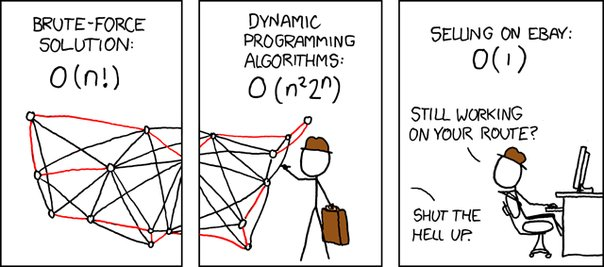
\includegraphics[width=0.48\textwidth]{compjoke.jpg}
  \end{center}
\end{wrapfigure}
Как введение в этот вопрос поговорим сначала о том, что такое логарифм. Ужасное слово? Вовсе нет. И какая разница, что его ``проходят в 11 классе''? Итак, попробуем вдохнуть жизнь в символ $\log_a b$. В данной записи $b$ называется {\it аргументом}, а $a$ --- {\it основанием}. Таким образом, для каждого $a$, $\log_a x$ --- это различная функция, то есть есть целое семейство логарифмов.

Так вот, $\log_a b$ есть степень, в которую нужно возвести $a$, чтобы получить $b$. Понятно? Если $a^x = b$, то $x = \log_a b$. Изи-бизи. Давайте здесь будем говорить про логарифм с основанием $a = 2$, но по сути в анализе сложностей основание логарифма роли не играет (скоро станет ясно, почему). 

{\bf Задача:} Вычислите $\log_3 27$, $\log_4 16$, $\log_{\sqrt{2}} 2$.

{\bf Задача:} Докажите, что $\log_c ab = \log_c a + \log_c b$, отсюда получите $\log_a b^n = n \log_a b$.

{\bf Задача:} Докажите, что $\log_a x = \log_c x / \log_c a$ (формула смены основания).

Логарифм --- очень медленно растущая функция. Её смысл в том, что если аргумент возводится в квадрат, фукция лишь удваивается. Скажем, если программа работает за $\log N$ операций, и на $N = 10^6$ (миллион) она работала 1 секунду, то на $N = 10^{12}$ (триллион) она будет работать две секунды. То есть, её практически по барабану на аргумент, и чем больше аргумент, тем больше ей по барабану.

Теперь обсудим, что же такое асимптотическая сложность $\mathcal{O}(\ldots)$. Обсуждать будем на всеми любимом алгоритме сортировки массива из $N \gg 1$ элементов. Какой алгоритм сортировки вы знаете? Реализуем наивный алгоритм.

{\bf Задача}: реализуйте алгоритм сортировки массива, пузырёк, выбор, whatever. Замерьте время исполнения на случайном массиве $N$ в зависимости от размера входа. 

Давайте произведём анализ сложности алгоритма сортировки, например, пузырьком. Один указатель $i$ бежит от $0$ до $N - 1$, другой $j$ бежит от $0$ до $j - 1$. Таким образом, всего мы встречаем $N (N - 1)$ пар элементов и тратим время $t_1$ на сравнение и время $t_2$ на перестановку элементов. Таким образом, полное время исполнения в худшем случае (пришлось переставить все элементы) равняется $N(N - 1) (t_1 + t_2)$.

Но это избыточно. Дело в том, что при $N \to +\infty$, $N^2 - N$ ведёт себя как $N^2$. Имеется в виду, что $N (N - 1) / N^2 \to 1$, асимптотически они ведут себя одинаково. Но ведь мы и хотим работать на больших входных данных. Поэтому заменим $N (N - 1)$ просто на $N^2$. И ещё нас не интересует множитель $t_1 + t_2$. Он зависит от архитектуры, языка программирования, от скорости ветра, он температуры процессора, от чего угодно. Поэтому просто выбросим его и будем писать $\mathcal{O}(N^2)$. Это единственная релевантная информация о сортировке пузырьком. Говорят, что он работает за квадратичное время (ибо $N^2$).

Есть другой алгоритм сортировки, быстрая сортировка. Вы знаете такие? Мой любимый --- merge sort.

{\bf Задание}: реализуем merge sort?

Сложность merge sort есть $\mathcal{O}(N \log N)$. Если учесть, что логарифм это почти мёртвая функция, то реально сортировка идёт почти линейное время, то есть почти такое же время, сколько нужно, чтобы просто прочесть массив. 

{\bf Задание}: почему я не пишу основание логарифма?

Давайте здесь поговорим об одном очень здоровском разделении задач в вычислительной теории. Оказывается, все задачи математики имеют очень чёткую структуру, о которой мы поговорим. Слышали ли вы что-либо про классы P и NP? Отлично, давайте поговорим об этом. Прежде чем начать говорить об этом, рассмотрим другую задачу.

Пусть есть $N$ городов, все соединены городами друг с другом. Есть стоимость проезда по каждой из дорог. Найти минимальную стоимость проезда из города $A$ и город $B$.

Есть и другая задача: пусть дано множество целых чисел $a_0, a_1, \ldots, a_N$. Можжно ли из них выбрать подмножество с нулевой суммой?

Оказывается, что задача (сегодня) решается не намного быстрее, чем за $\mathcal{O}(2^N)$. Другой пример, если есть число длины $N$, то оно факторизуется за время $e^{N^{1/3}}$. Оба этих времени --- ужасно огромные, самое ужасное, что это не полиномы. Раньше мы сталкивались с полиномиальными алгоритмами. Это алгоритмы сугубо неполиномиальные. Конечно, алгоритм --- это не характеристика задачи. Бывает, что долгое время думают, что задача не имеет быстрого решения, а она в конце концов имеет.

Класс $P$ (polynomial) --- это множество всех задач, для которых ответ можно найти за полиномиальное время. Класс $NP$ (nondeterministic polynomial) --- множество задач, для которых можно проверить ответ за полиномиальное время. 

Какие примеры задач из $P$? Например, сортировка. Мы находили решение почти за линейное время, которое полиномиально. Какая есть задача из $NP$? Например, задача факторизации. Если вам дали разложение числа длины $N$, то вы можете быстро (за полином от $N$ проверить, правильно разложение или нет). Опять же задача с поиском подмножества: если вам дали подмножество, мы без труда проверите, равна ли сумма нулю. А как с задачей поиска пути?

Очевидно, что класс $P$ содержится в $NP$ (почему?). Возникает вопрос, $P = NP$ или $P \neq NP$. За доказательство этого факта институт Клея предлагает приз в 1 миллион долларов (задача тысячелетия). Над этим вопросом бьются уже 30 лет, но ответа всё нет, хотя люди предполагают, что $P \neq NP$. Почему? Что бы значило равенство $P = NP$? 

Например, $NP$-задачи это доказательства теорем. Скажем, если мы работаем в какой-то формальной системе аксиом (аксиомы плоской геометрии, аксиомы Цермелло-Френкеля или что-нибудь другое), то теорема --- это лишь очень сложная комбинация аксиом. Стартуя от аксиом, найти теорему крайне сложно (этим из анимаются математики). Другое дело, если теорема уже сформулирована и дано доказательство, его очень просто проверить: нужно просто пройтись по доказательству и посмотреть,не противоречит ли оно аксиомам. Получается, что доказательство любой теоремы --- это задача из $NP$. Если $P = NP$, то значит, любую теорему можно за полиномиальное время вывести из аксиом на компьютере (полиномиально = быстро). Значит, все достижения Гаусса или Эйлера могли бы быть воспроизведены на домашнем компьютере (нужна просто умная программа, работающая с аксиомами).

Это очень сильное следствие равенства (недоказанного) классов $P$ и $NP$. Фейнман даже долгое время не верил, что их неравенство это открытая проблема. 

Можно ли развить этот разговор? Назовём задачу $NP$-трудной, если любая задача из $NP$ сводится к неё за полиномиальное время. Если к тому же эта задача сама лежит в $NP$, то мы зовём её $NP$-полной. Таким образом, $NP$-полные задачи образуют в некотором смысле подмножество ``типовых'' задач в классе $NP$: если для какой-то из них найден ``полиномиально быстрый'' алгоритм решения, то и любая другая задача из класса $NP$ может быть решена так же ``быстро''. 

Получается, достаточно всего {\it одной} задачи, которая вобрала бы в себя сложность всех $NP$ задач. Есть примеры таких задач, они явно построены и вполне реальны, одна из них 3SAT (QQ since Democritus). Таких задач уже тысячи, и найди мы решение хоть к одной из них, мы бы автоматически знали решение для всех задач из $NP$.  На самом деле это одна проблема в разных одеждах. 

Беда в доказательстве $P \neq NP$ в следующем. Известно очень много задач, которые лишь кажутся трудными. Истории известно множество примеров, когда задачу долгое время считали не имеющей решения за полиномиальное время, а потом решение это находилось. Поэтому чтобы действительно доказать $P \neq NP$, нужно взять $NP$-полную задачу (а не просто из $NP$) и доказать, что она не имеет решения за полиномиальное время. На данный момент этого не сделано. Наоборот, чтобы доказать, что $P = NP$, нужно взять любую $NP$-полную проблему и увидеть, что она имеет полиномиальное решение. Этого не сделано тоже :)


\section*{Тема 2: элементы теории чисел}
\subsection*{Немного об истории}
\begin{wrapfigure}{r}{0.5\textwidth}
  \begin{center}
    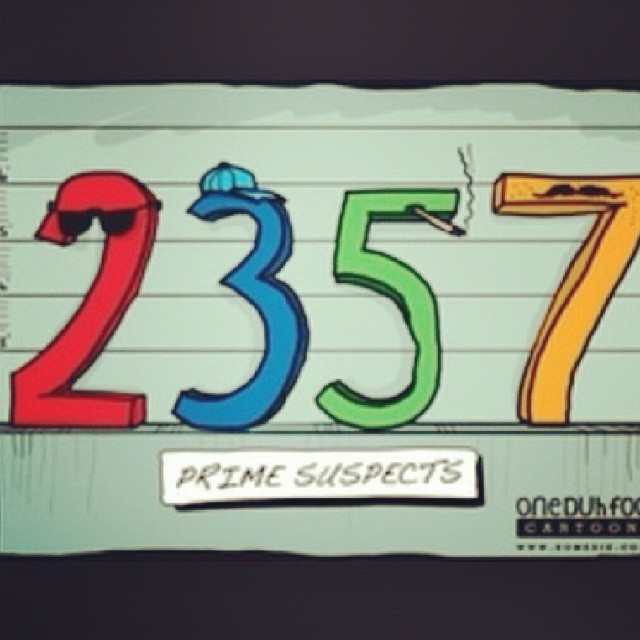
\includegraphics[width=0.48\textwidth]{primejoke.jpg}
  \end{center}
\end{wrapfigure}
Впервые понятие простого числа обсуждалось на папирусах древних египтян. Явным целенаправленным изучением занялись древние греки, в частности Евклид, который доказал бесконечность множества простых чисел (а вам же не слабо?), а также занудную (но безумно важную) теорему о том, что у любого числа есть единственное разложение на простые. Примерно в то же время было изобретено решето Эратосфена.

Во времена средневековья сильно ничего нового не изобрели (научились правильно креститься, разве что), пока в 17 веке не была сформулирована (а затем доказана Эйлером) малая теорема Ферма.

\begin{mfermat}
Если $p$ --- простое число, то для любого натурального числа $a$, $a^p = a\;\mbox{mod}\;p$.
\end{mfermat}

\begin{proof}
Проще всего доказать индукцией по $a$. База индукции $a = 0$ очевидна, $0^p - 0 = 0$. Теперь докажем приятное утверждение: $(x + y)^p = x^p + y^p$ для любых целых $x$ и $y$. По формуле бинома Ньютона, $(x + y)^p = \sum\limits_{i = 0}^p C^{i}_p x^i y^{p - i}$. Свойства коэффициентов таковы, что по модулю $p$ выживают только крайние два.

Таким образом, пусть мы знаем, что $k^p - k$ делится на $p$. Тогда $(k + 1)^p - (k + 1)$ по модулю $p$ есть $k^p + 1^p - k - 1$ = $k^p - k$, что уже делится на $p$. Шаг индукции доказан.
\end{proof}

\begin{proof}
Есть ещё второе доказательство, налядно-комбинаторное. Рассмотрим алфавит из $a$ символов и все строки длины $p$ в таком алфавите. Уберём из множества этих строк все строки вида $AAAAA$, состоящие из одного единственного символа. Во ставшемся множестве назовём строки дружественными, если они получаются циклическим сдвигом одна в другую, например, строки $AAABB$, $BAAAB$, $BBAAA$, $ABBAA$, $AABBA$ --- дружественные. Рассмотрим произвольную строку $S$ длины $|S|$. Сколько она имеет друзей? Чтобы ответить на этот вопрос, заметим, что строка $S$ не может быть конкатенацией нескольких одинаковых кусков $S \neq T + T + \ldots + T$, потому что длина $S$ --- простое число, и мы не рассмариваем строки вида $AAAAA$. Таким образом, сдвигая циклически строку $S$ можно получить её и ещё $p - 1$ её друзей. Других друзей у строки $S$ нет, поэтому всё множество строк разбивается на семейства размера $p$, поэтому $a^p - a$ делится на $p$.
\end{proof}

Вернёмся на время к истории. После доказательства малой теоремы Ферма Эйлер доказал, что ряд $$\sum\limits_{p_i < n} \frac{1}{p_i} = \log \log n + M,$$ то есть если брать ряд из обратных простых чисел, то он будет расходиться. То есть, если брать и суммировать обратные простые числа, то можно в сумме плучить любое сколько угодно большое число! Почему это удивительно? Вы наверняка знаете, что ряд из обратных натуральных чисел расходится, $$\sum \limits_{i = 1}^n = \log n + \gamma.$$ Нет? Давайте это докажем! Это очень просто. $$\frac{1}{2} + \frac{1}{3} + \frac{1}{4} + \ldots = \frac{1}{2} + \left(\frac{1}{3} + \frac{1}{4}\right) + \left(\frac{1}{5} + \frac{1}{6} + \frac{1}{7} + \frac{1}{8}\right) + \ldots < \frac{1}{2} + 2 \times \frac{1}{4} + 4 \times \frac{1}{8} + \ldots = \frac{1}{2} + \frac{1}{2} + \ldots.$$

Оказывается теперь, что если брать не все подряд идущие числа, а лишь простые, то тем не менее ряд будет расходиться, хоть и гораздо медленнее.

В начале 19 века была доказана теорема Лежандра-Гауса-Адамара. Пусть $\pi(n)$ --- число простых чисел, меньших $n$. Они показали, что $\pi(n) \sim n / \log n$, то есть при $n \to +\infty$ эти функции относительно почти не различаются. Получается, что простых чисел не так уж и мало, и по порядку величины $p_n = n \log n$, где $p_n$ --- $n$-тое простое число.

Зачем нам эта вся возня с простыми числами? Они отражают глубинную структуру любого числа. Это и даёт возможность использовать их в криптографии, в алгоритме RSA, который мы хотим побороть. 

В первую очередь, люди хотят, посмотрев на число, быстро определить, простое ли оно. Люди могут хотеть быстро раскладывать число на простые (как взломщик протокола RSA), а могут и просто заниматься поиском всех простых чисел меньших $n$.

\subsection*{Сопутствующие алгоритмы}
Какие мы знаем алгоритмы проверки числа $N$ на простоту? Самый простой, trial division --- делить число $N$ на все числа меньше него. Сколько работает такой алгоритм? А можно ли быстрее? Зачем делить именно до $N$? Есть и рандомизированный алгоритм, основанный на тесте Ферма. Его проходят почти все числа, кроме особенных чисел Кормихаэля.

В вопросе факторизации на классическом компьютере лучший результат: $\mathcal{O}(e^{\sqrt[3]{\log n}})$. Это довольно быстро, но всё равно видно, что алгоритм работает как экспонента от длины числа ($\log n$ --- по сути число знаков в числе). Если длина числа велика, то сложность растёт очень быстро.

Наконец, поговорим о поиске простых чисел, это делает модифицированное решето Эратосфена, которое работает за $\mathcal{O}(n \log \log n)$, то есть ищет все простые числа меньше $n$ за время, не сильно превышающее число операций, чтобы просто {\bf перечислить} эти числа от $0$ до $n$.

{\bf Задача}: реализуйте рандомизированный алгоритм проверки на простоту, основанный на матой теореме Ферма.

{\bf Задача}: реализуйте поиск всех простых чисел меньших $n$, используя модифицированное решето Эратосфена. Построим график числа операций от $n$?

\subsection*{Об алгоритме шифрования RSA}
\subsubsection*{Мотивация}
\begin{wrapfigure}{r}{0.5\textwidth}
  \begin{center}
    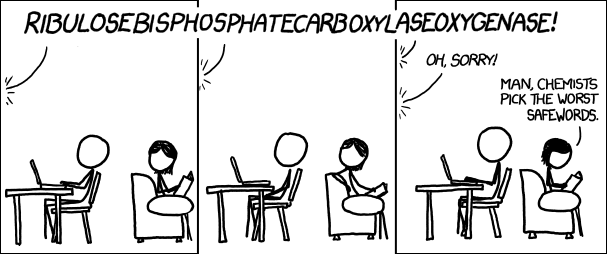
\includegraphics[width=0.48\textwidth]{cryptojoke.png}
  \end{center}
\end{wrapfigure}
А этом алгоритме нет совершенно ничего сложного. Даже вы с вашими друзьями можете без особого труда использовать его: он очень надёжен и прост. Так в чём же заключается суть алгоритма RSA? Пусть я хочу передать моему другу какое-то сообщение. Друга, кстати, зовут Александр. Пусть для простоты это будет большое-большое число $x$ (так или иначе все компьютерные сообщения это числа, текст тоже кодируется в число, как, например?). Александр (кстати, очень умный парень, занимается квантовой теорией поля и киральными эффектами) генерирует два простых числа $p$ и $q$ таких, что $p - 1$ и $q - 1$ не делятся на три. Он перемножает их и отправляет мне только число $N = pq$ по почте. Так как почте доверять нельзя, мы будем считать, что ключ может запросто быть перехвачен недоброжелателями. Поэтому и вообще можно считать, что Александр просто публикует число $N > x$ (которое, кстати, очень-очень-очень большое) где-нибудь у себя на страничке, например, в соцсети на стене.

Здесь становится ясно, зачем нам шифрование с открытым ключём. Если мы хотим шифроваться с закрытым ключём (который мы оба будем использовать при кодировании или декодировании), мы должны им как-то обменяться. Лучше всего это сделать в тёмном гараже или в тайге или в колодце, чтобы нас никто не увидел и не услышал. Чтобы наш ключ остался строго между нами. Но что делать, если Александр уедет в Принстон на PhD? Как тогда мне с ним встретиться? Мы должны как-то обменяться закрытым ключём. Но как сделать так, чтобы его не перехватили? Его нужно зашифровать! Но тогда нам нужен другой закрытый ключ, чтобы зашифровать первый. А как передать второй ключ! Тоже зашифровать! Ну... вы поняли.

\subsubsection*{Принцип шифрования и дешифровки}
Зная ключ Саши, я отправляю ему не $x$, а $x^3\;\mbox{mod}\;N$. Если злоумышленник перехватит $x^3\;\mbox{mod}\;N$, то в принципе он может восстановить $x$ (например, перебирая возможные $x$). Но так как $x$ --- очень большое число, то подбор займёт невероятно большое время. И нет на данный момент никакого хитрого алгоритма, который бы смог это сделать быстро (сильно быстрее, чем просто перебрать все $x$).

С другой стороны, Саша хранит у себя числа $p$ и $q$. В 1761 году была доказана теорема Эйлера. Она говорит, что если $a$ и $N$ --- взимно простые числа, то $a^{\varphi(N)} = 1\;\mod\;N$, где $\varphi(N)$ --- число всех чисел меньших $N$, которые с им взаимнопросты. Из этой теоремы тогда следует, что $x^{(p  - 1)(q - 1)} = 1\;\mbox{mod}\;N$ (ведь маловероятно, что $N$ делится на $x$, ведь так?).

Это означает, что последовательность $x\;\mbox{mod}\;N$, $x^2\;\mbox{mod}\;N$, $\ldots$, имеет период $(p - 1)(q - 1)$. Пусть нам удалось найти число $k$ такое, что $3k = 1\;\mbox{mod}(p - 1)(q - 1)$. Тогда $x$ можно восстановить так:
$$(x^3\;\mbox{mod}\;N)^k = x^{3 k}\;\mbox{mod}\;N = x\;\mbox{mod}\;N.$$

В последнем равенстве мы отбросили какое-то число $(p - 1)(q - 1) m$, чтобы получить чисто единицу, воспользовавшись периодичностью.

{\bf Задача}: докажите, что $(x^3\;\mbox{mod}\;N)^k = x^{3 k}\;\mbox{mod}\;N$.

На самом деле, мы поняли ещё не всё в быстрой дешифровке.

\subsubsection*{Поиск $k$}
Сначала разберёмся, как быстро решать уравнение $$3 k = 1\;\mbox{mod}\;(p - 1)(q - 1).$$ Мы уже поняли, что $(p - 1)(q - 1)$ не делится на три. Это уравнени эквивалентно записи $3k - (p - 1)(q - 1) l = 1$. Важно понять, что $1 = \mbox{gcd}(3, (p - 1)(q - 1)).$ Существует так называемый расширенный алгоритм Евклида, который позволяет решать уравнения $a x + y b = \mbox{gcd}(a, b)$ относительно $x$ и $y$. Это как раз наш случай: справа стоит единица, но ведь это и есть наибольший общий делитель коэффициентов $a = 3$, $b = (p - 1)(q - 1)$, а мы ходим найти $k$ и $l$.

Расширенный алгоритм Евклида действует следующим образом: определим величины $r_0 = a,\;s_0 = 1,\;t_0 = 0$, $r_1 = b,\;s_1 = 0,\;t_1 = 1$. Далее $r_{i + 1} = r_{i - 1} - q_i r_i$, $s_{i + 1} = s_{i - 1} - q_i s_i$, $t_{i + 1} = t_{i - 1} - q_i t_i$. Это уравнения в целых числах и всё определено. Когда получится $r_m = 0$, коэффициенты разложения будут $t_{m - 1}$ и $s_{m - 1}$.

Почему так? Для коэффициентов $r_i$ --- это обычный алгоритм Евклида. Из рекуррентного соотношения видно, что у $(r_{i - 1}, r_i)$ и $(r_{i}, r_{i + 1})$ один $\mbox{gcd}$. Значит, исходно он был $\mbox{gcd}(a, b)$, а в конце $\mbox{gcd}(r_{m - 1}, 0) = r_{m - 1} = \mbox{gcd}(a, b)$, то есть при переходе от одной пары остаткой к другой, наибольший общий делитель не меняется.

Что касается коэффициентов Безу, то можно явно проверить, что для $i = 0,\;1$ выполнено $a s_i + b t_i = r_i$. По индукции можно показать (покажите), что это держится для всех $i$. Получается, что на $m - 1$-ом шаге будет выполнено $a s_{m - 1} b t_{m - 1} = \mbox{gcd}(a, b)$ --- как раз то, что нужно!

Так как в плане остатков $r$ здесь всё работает так же как для обычного алгоритма Евклида, этот алгоритм также сходится очень быстро.

\subsubsection*{Теорема Эйлера}
Нам осталось для полного понимания доказать теорему Эйлера. 

\begin{euler}
Для взаимнопростых чисел $a$ и $N$, $a^{\varphi(N)} = 1\;\mod\;N.$.
\end{euler}

\begin{proof}
Рассмотрим множество чисел $a_1$, $a_2$, $\ldots$, $a_{\varphi(N)}$, которые взаимнопросты с $N$. Рассмотрим любое из них (обозначим его $c$). Во-первых для любого $a_i$, $c a_i = a_j\;\mbox{mod}\;N$, то есть $c$ домножением на $a_i$ переводит его в какой-то $a_j$ по модулю $N$ (верно, поскольку произведение взаимнопросто с $N$, и сколько из него не вычитай $N$, оно таким и останется). Во-вторых, если $c a_i = c a_j\;\mbox{mod}\;N$, то $a_i = a_j$, т.е. это просто одно и то же число (верно, так как в уравнении $c (a_i - a_j) = k N$ разность $a$ не может сократить всего $N$, а $c$ с ним взаимнопросто).

Поэтому при умножении всего множества на $c$, мы лишь переставляем в нём элементы (конечно, по модулю $N$), не склеивая их. Это всего лишь перестановка, биекция. Теперь справедливо следующее: $$\prod a_i = \prod c a_i\;\mbox{mod}\;N = c^{\varphi(N)} \prod a_i\;\mbox{mod}\;N.$$
Заметим, что произведение всех $a_i$ взаимнопросто с $N$, и его можно сократить. Мы тогда получаем $c^{\varphi(N)} = 1\;\mbox{mod}\;N$, теорема доказана.
\end{proof}

\subsubsection*{Итог}
Хотелось бы вкратце обсудить, чем же нам помогла факторизация на простые сомножители $p$, $q$. Почему без них задача очень трудна? Самое главное, что мы узнали тот самый период повторения, равный $(p - 1)(q - 1)$. Не зная $p$ и $q$, мы бы не смогли сделать то упрощение в самом начале. Без него, если $p, q \sim 10^{10000}$, то есть 10000-значные числа, отгадывание $x$ заняло бы миллионы лет. А имея это знание, мы можем сделать вычисления за время, линейно зависящее от длины числа $N$, то есть довольно быстро.
\section*{Тема 3: алгоритм Шора}
Теперь давайте начнём говорить об алгоритме Шора. На самом деле, основная часть алгоритма ясна и без квантового компьютера. Итак, алгоритм Шора хочет раскладывать число $N$ на простые сомножители за время, которое является полиномом от {\it длины} $N$, то есть на самом деле за $\mathcal{O}(\log^3 N)$. Снова отмечу, что $\log N$ по сути отражает длину числа $N$.

\subsection*{Подготовка}
Мы хотим найти для {\it нечётного} числа $N$ его делитель $1 < d < N$. Несколько замечаний:
\begin{enumerate}
\item Во-первых, если $N$ --- чётное, то тривиальный ответ $d = 2$, поэтому мы исследуем только нечётные числа. 
\item Далее, мы хотим, чтобы $N$ не было степенью простого числа, то есть $N \neq p^k$. Это можно очень быстро проверить: для всех $k < \log_2 N$ посмотреть на корень $\sqrt[k]{N}$ и убедиться, что он не простой. Корень вычисляется бинарным поиском аналогично за $\log_2 N$, каждый раз придётся возводить в степень $k$ за $\log k$, таким образом сложность этой проверки $\mathcal{O}(\log_2^2 N \log \log N)$. Теперь мы имеем нечётное $N$, не являющееся просто степенью простого числа. 
\item Кроме того, можно быстро проверить, является ли $N$ само по себе простым (рандомизированный алгоритм Ферма или что-то посложнее), с 2002 года это умеют делать за $\mathcal{O}(\log^3 N)$.
\end{enumerate}

\subsection*{Сведение проблемы факторизации к поиску порядка элемента}
Оказывается полезным переформулировать проблему факторизации $N$ в терминах другой задачи, которую эффективно решает квантовый компьютер. Что это за новая задача? Предположим, что нам каким-то образом удалось найти корень решения уравнения $x^2 = 1\;\mbox{mod}\;N$, отличный от тривиальных $1$ и $N - 1$. Перепишем уравение в виде $(x - 1)(x + 1) = 0\;\mbox{mod}\;N$. Если $x \neq 1$ и $x \neq N - 1$, то одна из скобок слева имеет с $N$ нетривиальный общий делитель (не равный $1$ и $N$). Таким образом, общий фактор есть $\mbox{gcd}(x - 1, N)$ или $\mbox{gcd}(x + 1, N)$, где $\mbox{gcd}$ означает greatest common divisor, наибольший общий делитель. 

Как же можно найти корень уравнения $x^2 = 1\;\mbox{mod}\;N$? 
\begin{enumerate}
\item Случайным образом выберём целое число $y$ между $0$ и $N - 1$. 
\item Проверим, что $\mbox{gcd}(y, N) > 1$. Если это так, то $N$ мы факторизовали $N$ и счастливы. Но такой редкой удачи скорее всего не произойдёт.
\item Теперь, когда $\mbox{gcd}(y, N) = 1$, мы уверены, что $y$ и $N$ взаимно-просты (coprimes). 
\item {\it Порядком} числа $y$ назовём такое наименьшее натуральное $r$, что $y^r = 1\;\mbox{mod}\;N$ ({\bf докажите}, почему он вообще существует? Не может быть так, что мы всё время умножаем, но никак не получаем 1 по модулю $N$)?
\item Если $r$ --- нечётное, то приходится вернуться к пункту $1$ и начать заново. К счастью, это происходит примерно в половине случаев. Это утверждение доказывается довольно громоздко, но идея в том, что вне зависимости от того, какое число мы раскладываем, при случайном выборе $y$ оно будет в половине случаев иметь чётный порядок, а в другой половине --- нечётный.
\item Итак, если $r$ --- чётное, то $x = y^{r / 2}$, и мы всё сделали.
\end{enumerate}

{\bf Задача}: найдите порядок $5^r = 1\;\mbox{mod}\;21$.

{\bf Задача}: докажите, что порядок не может быть больше $N$ ни при каких условиях.

\subsection*{Быстрый поиск $\mbox{gcd}$}
В прошлом пункте мы очень много ссылались на то, что мы ищем наибольший общий делитель очень быстро так, что это не отнимает времени, и вся сложность алгоритма высаживается на определении порядка элемента. Как же быстро искать наибольший общий делитель? Ответ был дан Евклидом (или кем-то до него, но Евлид знаменил тем, что издал огромный труд по математике, по сути объединив все достижения греков) и азывается алгоритмом Евклида.

Пусть, нужно найти $\mbox{gcd}(a, b)$, $a > b$. Рассмотрим остаток от деления $a$ на $b$, $a = k b + r$. Если $r = 0$, то $b$ --- и есть наибольший общий делитель, задача решена. Если нет, то сделаем следующие наблюдения:
\begin{enumerate}
\item Если какое-то число делит $a$ и $b$, то оно делит $r$.
\item Не может такого быть, что какое-то число делит $r$ и $b$, но не делит $a$.
\end{enumerate}
Таким образом, наибольший обещий делитель $a$ и $b$ (назовём его $d$) делит $r$ и является общим делителем $b$ и $r$. Могут ли $b$ и $r$ иметь общий делитель больше чем $d$? Нет! Потому, что тогда он должен будет делить и $a$ тоже, но мы уже сказали, что $d$ --- наибольший общий делитель $a$ и $b$. Отсюда можно заключить, что $\mbox{gcd}(a, b) = \mbox{gcd}(b, r)$. Впечатлены? 

Таким образом, нужно итеративно спускаться от исходной задаче к дальнейшим, используя алгоритм Евклида, пока мы не получим $r = 0$. Сколько операций это у нас займёт, если $a$ и $b$ очень велики? Заметим, что каждый раз, когда мы переходим от $a, b$ к $b, r$, правый аргумент уменьшается как минимум вдвое (остаток не может быть больше чем $b / 2$, почему?). Раз так, то правый аргумент достигнет единицы за $\mathcal{O}(\log N)$ операций. Надо отметить, что каждое вычисление остатка тоже требует порядка $\mathcal{O}(\log N)$ операций, и в дополнение если $N$ очень велико, то умножения чисел такого порядка делаются за $\mathcal{O}(\log N \log \log N)$, поэтому итоговая сложность поиска нибольшего общего делителя всего лишь $\mathcal{O}(\log^3 N \log \log N)$.

{\bf Задача}: почему умножать длинные числа можно именно за такое время? Почему для поиска остатка нужно такое количество операций?

{\bf Задача}: реализуйте алгоритм Евклида. На случайных числах проверьте асимптотику времени его работы. Хватит ли для этого стандартных целочисленных типов? Как с этим можно побороться? 

{\bf Задача}: каков самый наивный алгоритм поиска наибольшего общего делителя? Какова его сложность? Сильно медленнее ли о работает?

\section*{Тема 4: комплексные числа}
\begin{wrapfigure}{r}{0.5\textwidth}
  \begin{center}
    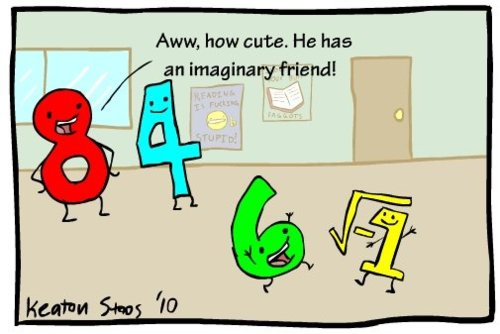
\includegraphics[width=0.48\textwidth]{complexjoke.jpg}
  \end{center}
\end{wrapfigure}
Пифагорейцы построили религию, одним из ключевых моменов которой было понятие числа. Какого числа? В сегодняшних терминах они оперировали только рациональными числами, $p / q$ и всё такое. Есть легенда, что когда один из последователей Пифагора смог доказать, что в прямоугольном треугольнике с катетами $1$ и $1$ диагональ не является рациональным числом (можешь доказать?), его выбросили за борт, дабы он не рушил их стройную картину мира. Мы же не собираемся так делать?

Легко представить себе натуральные числа. Чуть сложнее --- рациональные. Но на мой взгляд, иррациональные числа --- это большая мистика. Как отрезать от пирога $1 / \pi$-долю? Любой человек начнёт приближать $1 / \pi$ снизу и сверху рациональными дробями со сколь угодно хорошей точностью. Таким образом, сам по себе концепт вещественного (иррационального) числа не так уж интуитивен. Но мы во всю их используем!

Давайте нашу смелость распространим на следующее поле чисел: к{\bf о}мплексные числа. Стандартное определение: это числа вида $z = x + i y$, где $x$ и $y$ --- привычные вещественные числа, а $i$ --- некий символ такой, что $\boxed{i^2 = -1}$. Что за ерунда? А теперь представьте себя в каменном веке, и вам говорят, что $-1 \times -1 = 1$. Докладчик едва бы ушёл от вас живым. Что за $-1$? Это сколько на пальцах? Так же, как люди смирились с отрицательными и иррациональными числами, можно смириться и с символом $i$. Тем более, что природа описывается именно комплексными числами (а иногда и кое-чем посложнее).

{\bf Задача:} пусть $z_1 = x_1 + i y_1$, $z_2 = x_2 + i y_2$. Запиши выражения для $z_3 = z_1 \times z_2$, $z_3 = z_1 \pm z_2$, $z_3 = z_1 / z_2$ (для этого тебе потребуется подсказка: $1 / (a + i b) = (a - i b) / (a^2 + b^2)$ --- докажи сначала её).

Как лучше всего себе представлять такие числа? Вещественные числа мы рисуем на прямой. А комплексные числа, коли они задаются парой вещественных чисел, представляют векторами на двумерной комплексной плоскости. Если $z = x + i y$, то ось $x$ называется {\it вещественной осью} $\mbox{Re} z$ (действительно, $x$ входит в $z$ без странного символа $i$), а ось $y$ называется {\it мнимой осью} $\mbox{Im} z$(не находите это определение немного дискриминирующим?). Как вы уже догадались $\mbox{Re}$ ознавачает real, а $\mbox{Im}$ --- imaginary.
Привожу рисунок, где почему-то $x$ и $y$ обозначены как $a$ и $b$, простим автора сего рисунка.

\begin{center}
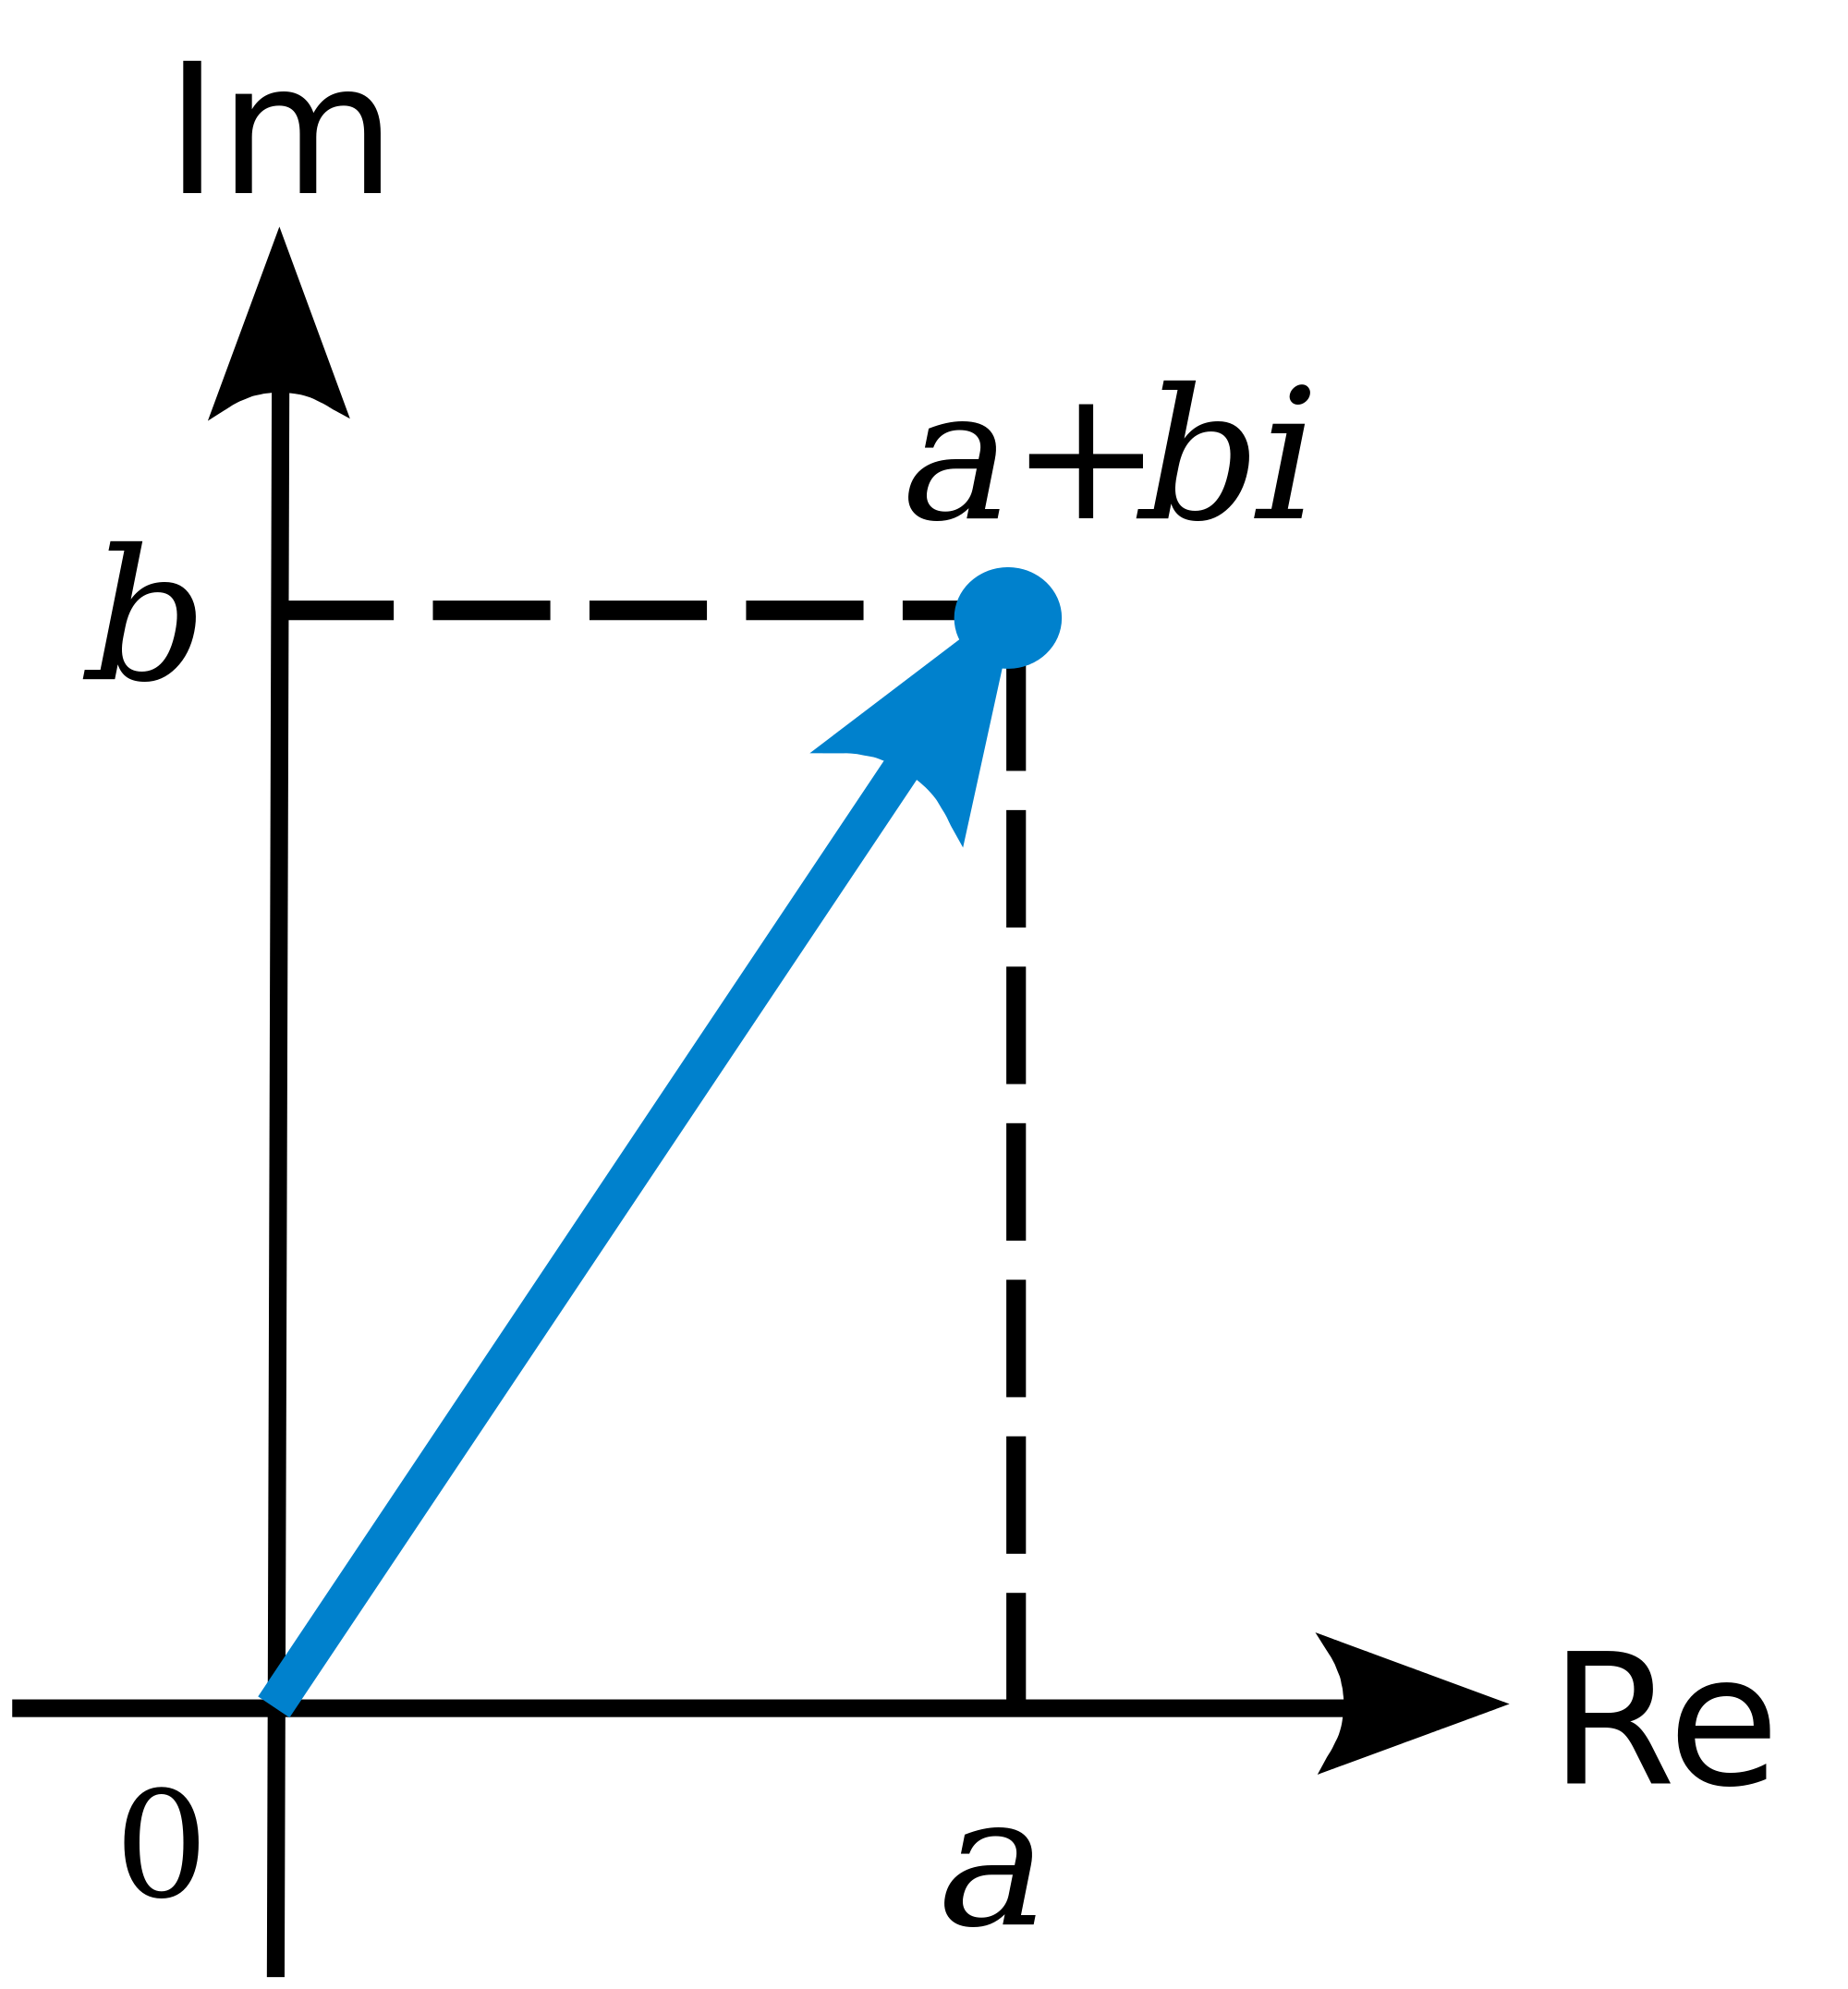
\includegraphics[scale=0.1]{cn_plane.png}
\end{center}

{\bf Задача:} возьмём прошлую задачу. Теперь представьте, что $z_1$, $z_2$ --- вектора на комплексной плоскости (представлять и не нужно, они {\it есть} вектора). Что из себя представляют {\it геометрически} эти действия над комплексными числами?

Запись $z = \mbox{Re} z + i \mbox{Im} z$ называется алгебраической формой записи комплексного числа. само название говорит, что она не очень удобна. Пойдём дальше. Раз у нас есть вектор на плоскости, почему бы не сказать, что у него есть длина и некий угол поворота относительно оси $x$? Снова всё прояснит рисунок.

\begin{center}
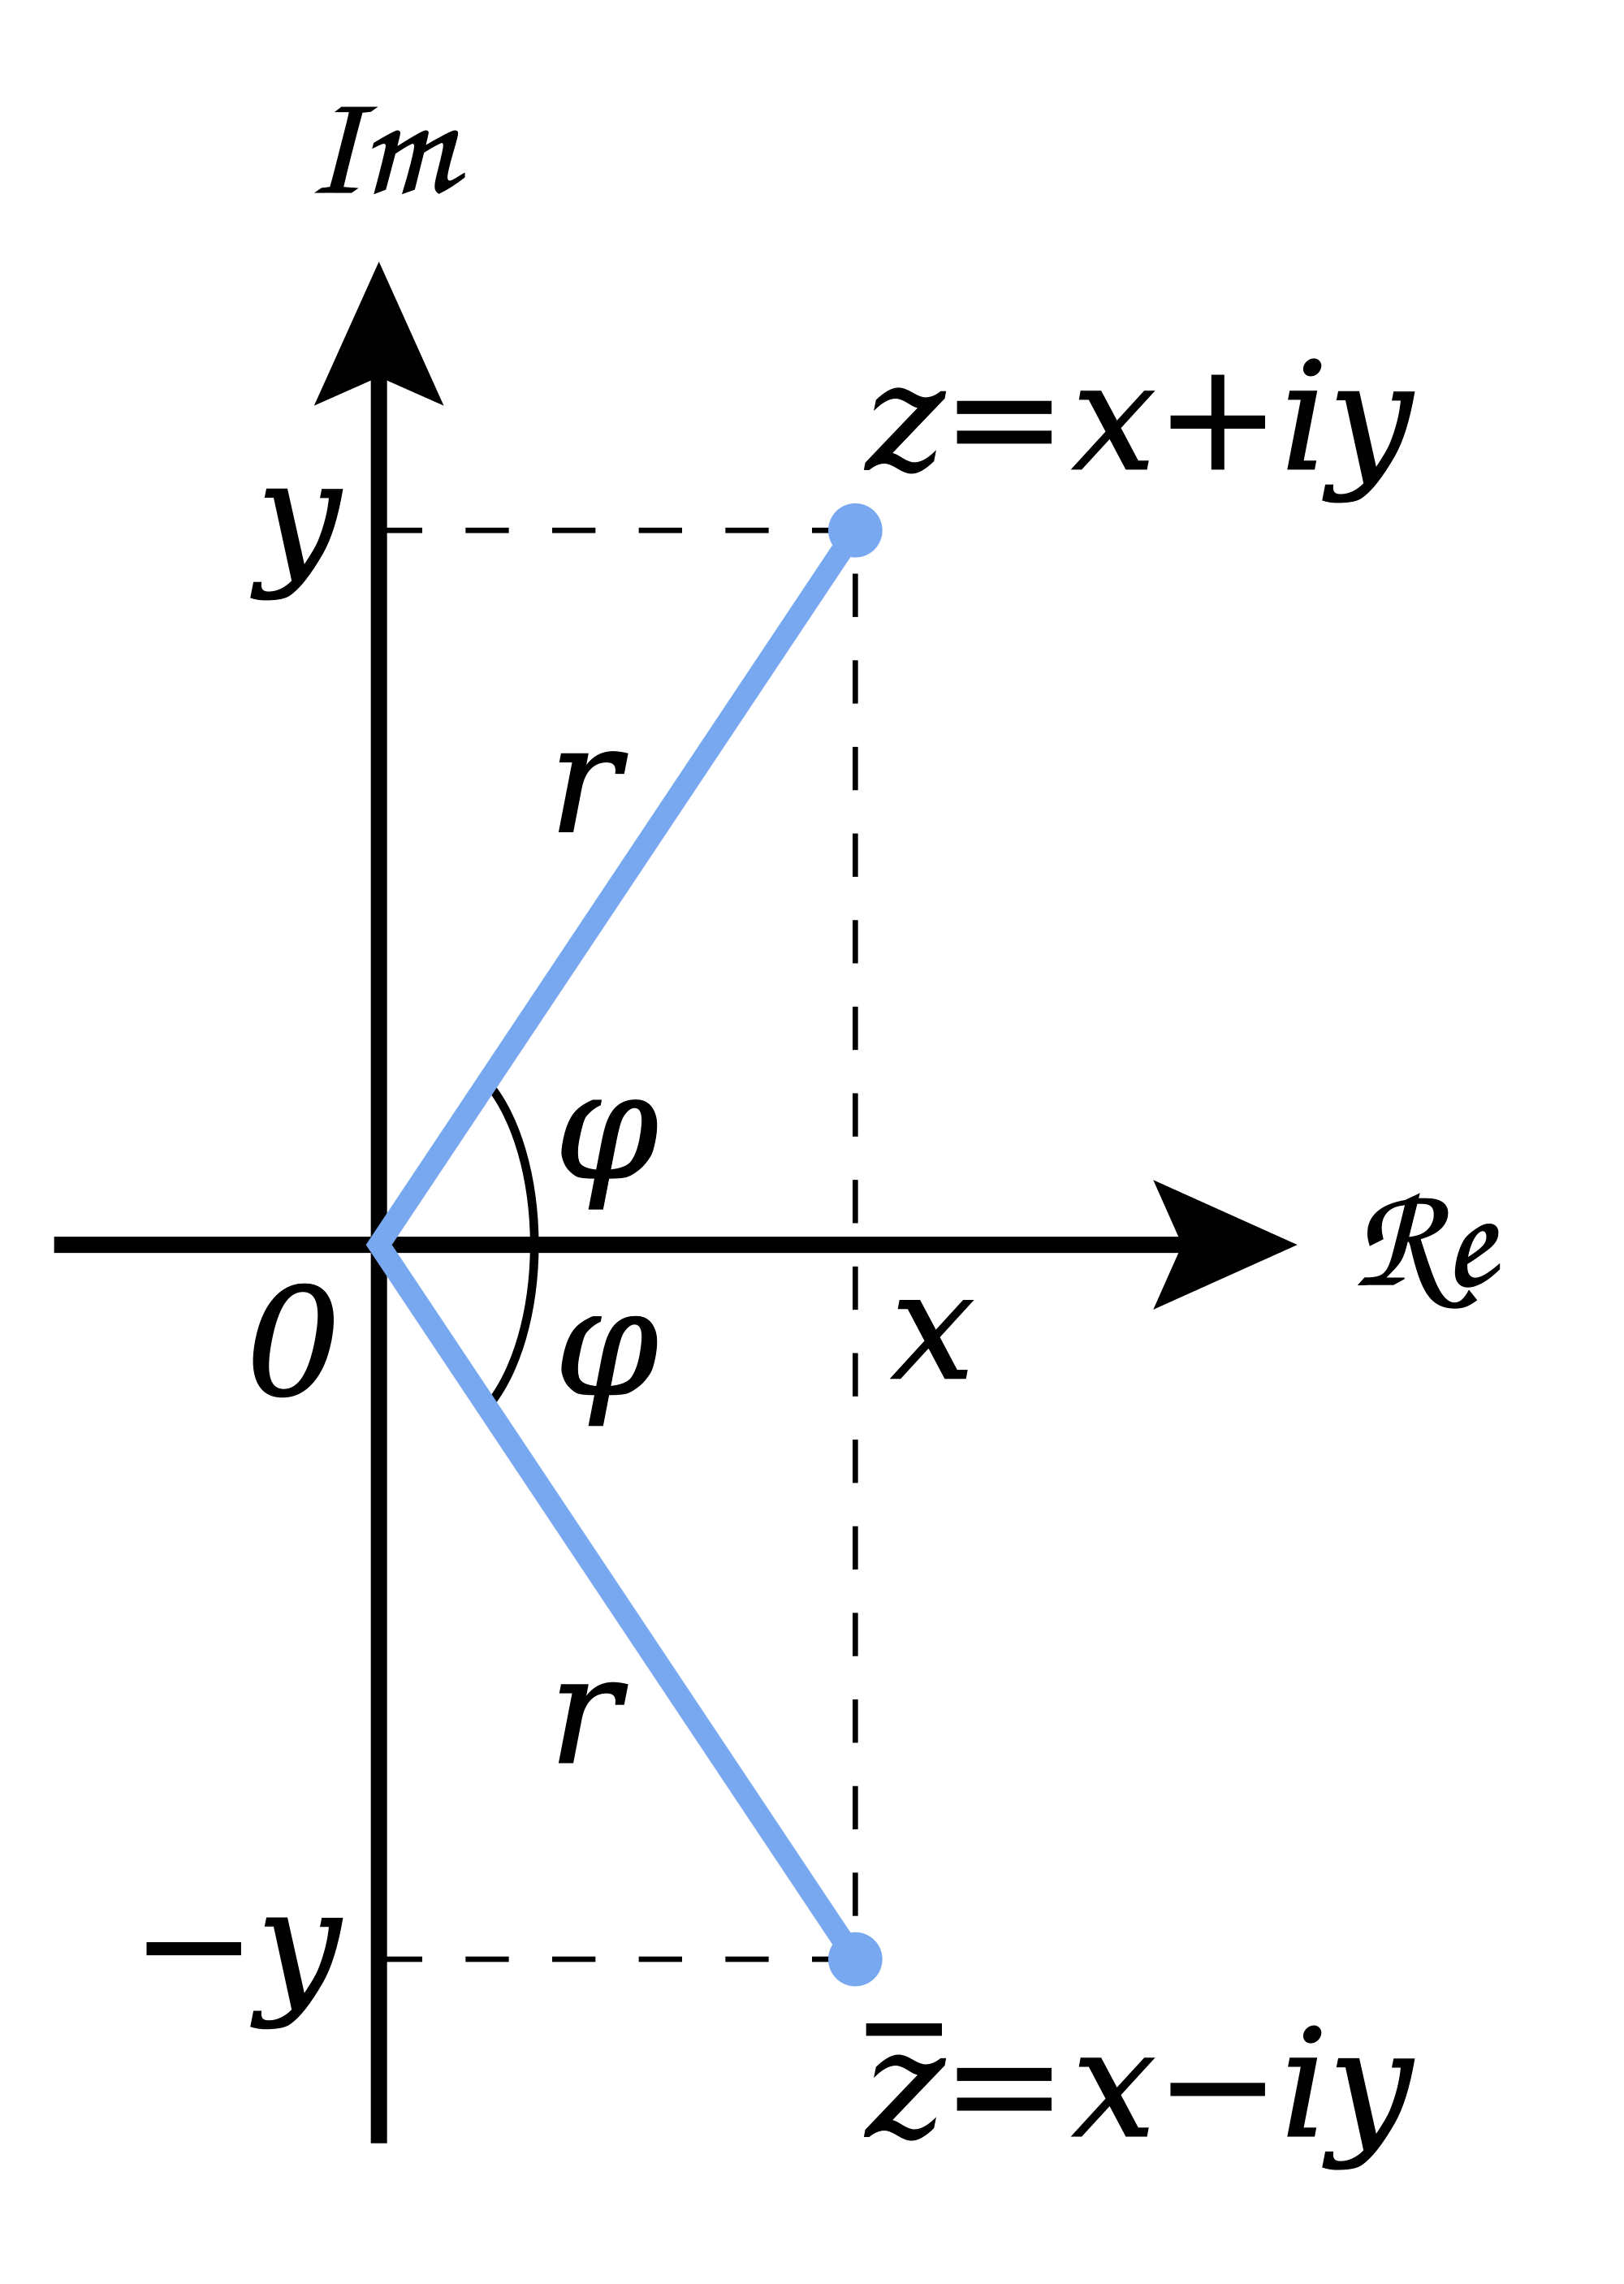
\includegraphics[scale=0.1]{cn_plane_phi.png}
\end{center}

Отлично! Получается, что $x = r \cos \varphi$, $y = r \sin \varphi$! И мы напишем $z = r \left( \cos \varphi + i \sin \varphi \right)$. Эта приятная запись называется тригонометрической формулой записи комплексного числа.

{\bf Задача:} зная $x$ и $y$, найди $r$ и $\varphi$.

{\bf Задача:} пусть $z_1 = r_1 \left( \cos \varphi_1 + i \sin \varphi_1 \right)$, $z_2 = r_2 \left( \cos \varphi_2 + i \sin \varphi_2 \right)$. Тогда $z_3 = r_3 \left( \cos \varphi_3 + i \sin \varphi_3 \right) = z_1 \times z_2$ или $z_1 \pm z_2$ или $z_1 / z_2$. Найди выражения для $r_3$ и $\varphi_3$.

{\bf Задача:} снова попробуй понять, что же происходит на плоскости геометрически при этих операциях?

{\bf Задача для тру пацанов:} Зная $z = r \left( \cos \varphi + i \sin \varphi \right)$, найти $z^n$ (если прошлые задачи решены, то эта должна поддаться в полтычка).

Введём ещё пару полезных обозначений. Если $z = x + i y$, то $\bar{z} = x - i y$, называется комплексным сопряжением.

{\bf Задача:} чему это соответствует геометрически?

{\bf Задача:} Что происходит с параметрами $r$ и $\varphi$ при сопряжении?

Очень важное обозначение --- модуль числа $|z|$, по сути длина. 

{\bf Задача:} докажи, что $|z|^2 = z \bar{z}$. Теперь понятно, почему $1 / (a + i b) = (a - i b) / (a^2 + b^2)$?

Наконец, мы подошли к самому соку. Я не буду приводить доказательство этого факта (достаточно лишь знать, что его сделал Эйлер), однако если кому-то хочется, я могу его привести, это очень и очень красиво. Так вот, эта формула заслуживает отдельного места: $$\boxed{e^{i \varphi} = \cos \varphi + i \sin \varphi}.$$

Чтоооо!?!? Что за экспонента от мнимого числа (угла)? есть один хороший способ это определить. Когда мы говорим про экспоненту вообще, мы имеем в виду $e^x = 1 + x + x^2 / 2! + \ldots + x^n / n! + \ldots$. Это ряд, который сходится для всех $x$. А теперь просто уместо $x$ подставим сюда $i \varphi$, и нет проблем. Главное, что экспонента остаётся экспонентой, то есть сохраняет своё чудесное свойство $e^x e^y = e^{x + y}$.

Благодаря этой супер-формуле (которая, кстати, носит имя Эйлера и утверждает, например, что $e^{i \pi} = -1$), мы переписываем алгебраическую форму в виде экспоненциальной формы, самой прогрессивной и успешной: $r \left( \cos \varphi + i \sin \varphi \right) = r e^{i \varphi}$. Таким образом, вся структура комплексного числа у нас теперь как на ладони. Вот есть длина $r$, а есть как-бы направляющий множитель $e^{i \varphi}$.

{\bf Задача}: пусть $r = 1$, что такое множество точек $z = 1 \times e^{i \varphi}$? Хорошенько почувствуйте, что такое это за экспонента. Докажите, что $|e^{i \varphi}| = 1$.

{\bf Задача}: снова посмотрим на операции деления и умножения $z_1 \times z_2$ и $z_1 / z_2$. Экспоненциальная форма записи просто {\it создана} для того, чтобы делить и умножать. Поделите и умножьте, здорово получается?

{\bf Задача}: может, вы устали от абстрактных общих формул? Вот такая задача: $z_1 = 3 + 4i$, $z_2 = -2$. Найдите $r_1, \varphi_1, r_2, \varphi_2$, запишите экспоненциальную форму обоих чисел, изобразите оба числа на комплексной плоскости. Вычислите $z_2 / z_1$, работая сначала в алгебраической, затем в экспоненциальной форме.

После того, как нам стала известна экспоненциальная форма записи, мы готовы начать искать корни из комплексных чисел. Тьфу, что может быть интересного в поиске корня? Ну-ка, чему равен корень из $i$? сколько их? В общем, вся соль в том, что $e^{2 \pi i} = 1$, $e^{4 \pi i} = 1$, и вообще $e^{2 k \pi i} = 1$ для любого $k$. В вопросе извлечения корня это имеет очень глубокие последствия. 

Будем считать, что мы извлеккаем корень из числа $z = r e^{i \phi}$ (то есть, из любого числа). Очевидно, что если взять $w = r^{1/n} e^{i \phi / n}$, то $w^n = z$ (здесь $r^{1/n}$ подразумевается как самый обычный школьный корень без понтов). То есть, $w$ --- корень. Это всё? Нет! Ведь $w \times e^{2 i \pi / n}$ --- тоже корень (проверьте). Так же как и любое число $w \times e^{2 i \pi k / n}$. Сколько различных $k$ надо брать? Можно видеть (увидьте!), что при $k = 0, \ldots, n - 1$ мы будем получать различные корни, а дальше корни будут накладываться на старые.

Поэтому всего уравнение $w^n = z$ имеет $n$ корней вида $$w_k = r^{1/n} e^{i \varphi / n + 2 \pi i k / n}.$$

{\bf Задача}: что из себя представляют корни на плоскости? Что это за фигура? Рассмотрите $w^3 = 1$ для определённости, нарисуй корни на комплексной плоскости.

Рассмотрим $z = 1$ и уравнение $w^n = 1$. Корни этого уравнения --- т.н. корни из единицы, очень известная конструкция. Ясно ли, что $w_k = e^{2 \pi i k / n}$? Изобразите это семейство на плоскости.

\begin{center}
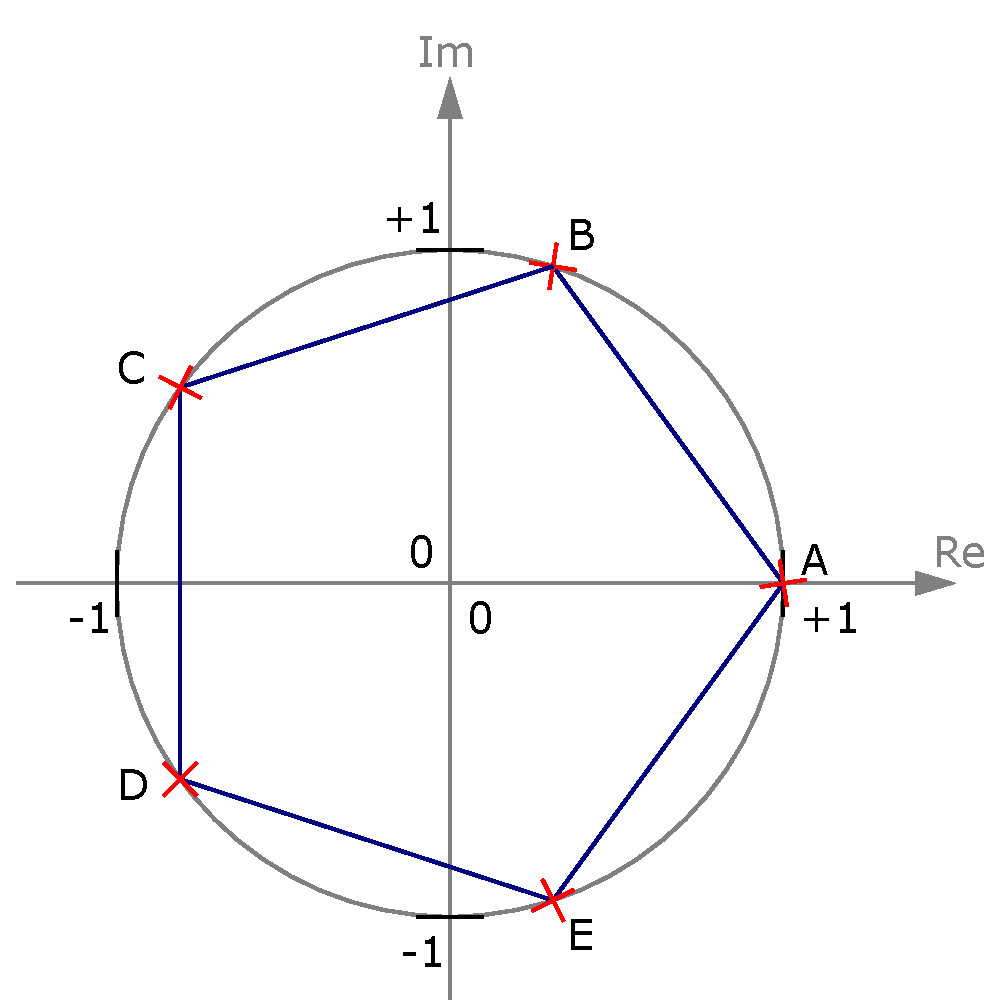
\includegraphics[scale=0.7]{roots.pdf}
\end{center}

{\bf Задача}: решите уравнение $z^2 + z + 4 = 0$.

\section*{Тема 5: Дискретное преобразование Фурье}
\subsection*{Определение ДПФ и задачи}
\begin{wrapfigure}{r}{0.5\textwidth}
  \begin{center}
    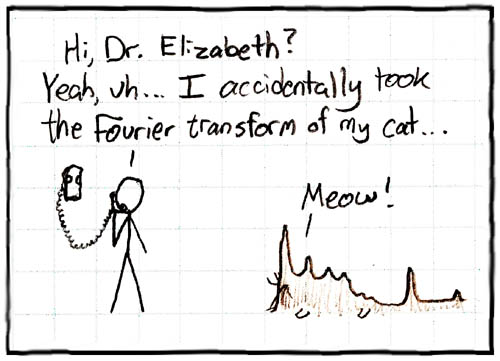
\includegraphics[width=0.48\textwidth]{fourierjoke.jpg}
  \end{center}
\end{wrapfigure}
Вот мы и дошли до концепции дискретного преобразования Фурье. Пожалуй, это мощнейший инструмент для решения очень большого класса задач. Когда мы слушаем музыку, мы смотрим на такую полосочку, где показывается вклад различных частот в песню, настраиваем его эквалайзером. Что означает этот ``вклад частоты''? Ещё вопрос, как работают программы вроде SoundHound, которые определяют трек по огромной базе данных? а все эти вопросы даёт ответ частотный анализ, а именно преобразование Фурье. Для начала определим, что же такое преобразование Фурье.

Пусть есть функция $f(n)$, определённая в целых точках $n = 0, 1, \ldots, N - 1$. Можно себе это представлять как функцию, определённую на точках решётки. Кроме того обычно накладывается условие $f(0) = f(N)$ (то есть цепочка замкнута в кольцо). Это условие не играет роли для больших $N$. Можно считать, что $f(n)$ --- это записанная амплитуда звуковых колебаний от времени $n$ (сделанная в некоторых временных точках). Идея заключается в том, что нам нужно ``свернуть'' функцию с комплексной экспонентой определённой частоты, чтобы как раз найти вклад этой самой частоты в звук. 

Рассмотрим множество частот, $k_m = 2 \pi m / N$, $m = 0, \ldots, N - 1$. Эти частоты именно такие, чтобы обеспечить наложенное выше граничное условие. Только эти частоты и дают вклад. Опять же видно, что при больших $N$ этих частот бесконечно много и они уже почти непрерывны.

Таким образом, $$\hat{f}(m) = \frac{1}{\sqrt{N}} \sum\limits_{x = 0}^{N - 1} e^{i k_m x} f(x).$$ Что произошло? У нас имелась функция $f(x)$ (амплитуда звука), определённая в $N$ точках. А мы хотим получить {\it спектр} этой функции $\hat{f}(m)$, где $m$ --- уже индекс частот, которых тоже $N$ ($m$ нумерует частоты $k_m = 2 \pi m / N$. Чтобы найти $m$-тый спектр, нужно вычислить упомянутую выше сумму. Это и будет вклад частоты $k_m$ в данный сигнал. Если $\hat{f}(m)$ --- велика по сравнению с остальными частотами, то человек слышит звук примерно частоты $k_m$.

Вы заметили, что $\hat{f}(m)$ стало комплексной величиной?

{\bf Задача}: докажите центральное тождество, $\frac{1}{N} \sum\limits_{x = 0}^{N - 1} e^{i k_m x} = \delta_{m, 0}$, где $\delta_{a, b}$ --- символ Кронекера, равен 0 всегда, когда $a \neq b$, иначе 1. Аналогично $\frac{1}{N} \sum \limits_{m = 0}^{N - 1} e^{i k_m x} = \delta_{x, 0}$.

{\bf Задача}: используя центральное тождество, докажите, что $f(x) = \frac{1}{\sqrt{N}} \sum\limits_{m = 0}^{N - 1} e^{-i k_m x} \hat{f}(m).$ (формала обратного преобразования Фурье, т.е. от спектра к сигналу).

{\bf Задача}: для функции $f(0) = 0$, $f(1) = 1$, $f(2) = 2$ ($N = 3$) найдите Фурье-спектр. Имея спектр, проведите обратное преобразование Фурье, т.е. снова восстановите сигнал.

{\bf Задача}: задача про старателей.

{\bf Задача}: про пьяницу.

\subsection*{Алгоритмическая сторона вопроса}
Какое время требуется, чтобы вычислить спектр функции? Казалось бы, нужно найти $N$ сумм по $N$ слагаемых, и сложность алгоритма будет $\mathcal{O}(N^2)$ (в каких классах лежит эта задача?) Но можно сделать ещё быстрее, оказывается, существует алгоритм, работающий за $\mathcal{O}(N \log N)$, то есть опять же почти что линейное время. Прежде чем рассказывать про этот алгоритм, давайте обсудим применения преобразования Фурье в компьютерных науках. По сути, основное применение --- это перемножение длинных чисел (или строк), которое применяется в таких задачах, как поиск подстроки, поиск соответствия, да и просто в алгоритмах быстрой арифметики.

Ранее я упоминал, что два числа, длина которых равна $N$, можно перемножить за $\mathcal{O}(N \log N)$. Это очень важно при работе с большими числами, например в криптографии или опять же при перемножении строк для поиска соответствий. Быстрое преобразование Фурье --- ключ к такой скорости. 

Как же умение находить какой-то непонятный спектр вообще нам поможет перемножить два длинных числа? Сначала давайте скажем, что мы перемножаем не два числа, а два мноочлена $P_a(x) = a_{n - 1} x^{n - 1} + \ldots + a_0$ и $P_b(x) = b_{n - 1} x^{n - 1} + \ldots + b_0$.

{\bf Задача}: показать, что перемножение многочленов и чисел это одно и то же. Нет, ну правде ведь одно и то же, за исключением переносов в другой разряд, но это легко можно допилить.

\subsection*{Перемножение многочленов, чисел и т.д.}

Всё, теперь мы хотим перемножить два многочлена, а не два числа (видно, что задачи сводятся друг к другу за время порядка линейного). Как перемножать многочлены наивно? Надо подумать, какие слагаемые дадут вклад в каждую из итоговых степеней и всё просуммировать. В итоге снова получается $\mathcal{O}(N^2)$ операций, что не удивительно: ничего нового пока что мы не изобрели. 

Теперь переформулируем это немного на другой язык. Обозначим $\omega = e^{2 \pi i / 2N}$. То есть элементарный корень из единицы степени $2 N$ (заметим, что итоговый многочлен будет степени $2 N$). Все другие корни из единицы --- это степени $\omega$: $\omega^0$, $\omega^1$, $\ldots$, $\omega^{N - 1}$. Предположим, что каким-то чудом нам стали известны значения $P_a(\omega^k)$ и $P_b(\omega^k)$ (то есть мы знаем значения обоих начальных многочленов во всех корнях из единицы). Тогда мы автоматически знаем их произведение во всех точках $P_a(\omega^k) P_b(\omega^k)$. Зачем нам это нужно? Многочлен $P_c = P_a P_b$ --- степени $2N$. Теорема Лагранжа (какая из?) гарантирует, что если нам известно значение многочлена степени $2 N$ в $2 N$ точках, то коэффициенты восстанавливаются всегда и однозначно. Следовательно, нам нужно узнать значения $P_c(\omega^k) = P_a(\omega^k) P_b(\omega^k)$.

\subsection*{Прямое Фурье}
Первое, что нужно сделать, это посчитать значения $P_a(\omega^k)$. Дополним многочлен $P_a$ до степени $2 n$ нулевыми коэффициентами. Тогда 

\begin{gather*}
P_a(\omega^k) = a_{n - 1} \omega^{kn - k} + c_{n - 2} \omega^{kn - 2k} + \ldots + a_0 =  \sum\limits_{\alpha  = 0}^{2 n - 1} a_{\alpha} e^{2 \pi i k \alpha / 2 n} = \hat{P_a}(k).
\end{gather*}

Вот это сюрприз! Да ведь это формула прямого преобразования Фурье! Не видите? В последнем выражении $a_{\alpha}$ --- это сигнал, $2 \pi k / 2n = p_k$ --- это частота. Получается, в экспоненте стоит $i p_k \alpha$, как и подобает. Получается, если мы вычисляем многочлен $P_a$ в точке $\omega^k$, мы получаем преобразование Фурье сигнала, если за сигнал считать последовательность его коэффициентов! На самом деле не хватает множителя $1 / \sqrt{N}$, о это всего лишь множитель, who cares? 

\subsection*{Поточечное произведение}
После того, как мы посчитали значения $P_a(\omega^k)$ и $P_b(\omega^k)$, для всех $k$ найдём поточечное произведение $P_c(\omega^k) = P_a(\omega^k) \times P_b(\omega^k).$
\subsection*{Обратное Фурье} 
Теперь мы знаем спектр многочлена $P_c(\omega_k)$, то есть спектр сигнала, если за сигнал принять его коэффициенты. Отсюда, используя центральное тождество, мы в состоянии восстановить сами коэффициенты! 
$$c_{\alpha} = \frac{1}{2 n} \sum\limits_{k = 0}^{2 n - 1} e^{-2 \pi i k \alpha / 2 n} \hat{P_c}(k) = \frac{1}{2 n} \sum \limits_{k = 0}^{2 n - 1} \omega^{-\alpha k} \hat{P_c}(k).$$

Это ведь всего лишь обратное преобразование Фурье от спектра. В итоге нам нужно: сначала для многочленов $P_a$ и $P_b$ сделать преобразование Фурье от их коэффициентов, затем поточечно их умножить и произвести обратное преобразование Фурье. Всё это хорошо изображено на следующей схеме:

\begin{center}
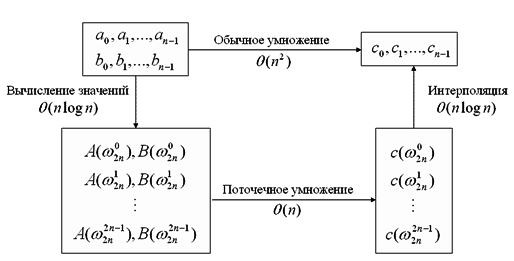
\includegraphics[scale=0.7]{schem.png}
\end{center}

{\bf Задание}: реализуйте этот алгоритм с медленным преобразованием Фурье.

\subsection*{Быстрое преобразование Фурье}
Как видно, наш алгоритм опирается на то, что мы умеем делать Фурье быстро. То есть, если бы мы могли делать Фурье за обещанные $\mathcal{O}(N \log N)$, мы бы могли перемножать очень длинные числа очень быстро и делать ещё очень много разных прикладных задач. Но вот вопрос: как же вычислять те огромные ужасные суммы не за $\mathcal{O}(N^2)$? Ответ дал Гаусс ещё в 1805 году, когда исследовал орбиты движения планет. К сожалению, в то время это был не очень-то актуальный вопрос (спросите меня про эпициклы, пожалуйста, спросите меня про эпициклы!). Метод переоткрыли в 1965 году Тьюки и Кули.

В чём основная соль метода? В основе лежит так называемся doubling trick. По сути, это очень похоже на merge sort, идея та же: разделяй и властвуй. Здесь и далее считаем, что многочлен имеет степень, равную степени двойки, $n = 2^k$.

Заметим, что для любого $x$, $A(x) = a_0 + a_2 x^2 + a_4 x^4 + \ldots + x (a_1 + a_3 x^2 + \ldots) = A_0(x^2) + x A_1 (x^2)$. Теперь многочлен $A_0(x)$ содержит в себе чётные коэффициенты, а $A_1(x)$ --- нечётные. Предположим, что мы хотим вычислить значения многочлена $A(x)$ в на $n$ корнях из единицы, т.е. сделать преобразование Фурье. 

Пусть для многочленов $A_0(x)$ и $A_1(x)$ уже сделано преобразование Фурье, т.е. найдены значения $A_0(\omega_{n / 2}^k)$, $A_1(\omega_{n / 2}^k)$, $k = 0, \ldots, n / 2 - 1$. По определению корня из единицы $\omega_{n / 2}^k = \omega_{n}^{2 k}$. Таким образом, $$A(\omega_{n}^k) = A_0((\omega_n^k)^2) + \omega_n^k A_1((\omega_n^k)^2) = A_0(\omega_{n / 2}^k) + \omega_n^k A_1 (\omega_{n / 2}^k),\; k < n/2.$$
А для $k \geq n / 2$ мы имеем $$A(\omega_{n}^{k + n/2}) = A_0((\omega_{n}^{k + n/2})^2) + \omega_{n}^{k + n/2}  A_1((\omega_{n}^{k + n/2})^2) = A_0((\omega_n^k)^2) - \omega_n^k A_1((\omega_n^k)^2) = A_0(\omega_{n / 2}^k) - \omega_n^k A_1(\omega_{n / 2}^k).$$

Таким образом, если мы вычислили преобразование Фурье для двух подмногочленов, преобразование для полного лепится за $n$ шагов. Таким образом, уравнение на сложность имеет вид $T(n) = 2 T(n / 2) + \alpha n$, решением которого является $\mathcal{O}(n \log n)$.

\section*{Тема 6: пара слов о линейной алгебре}
Сейчас мы поговорим о линейной алгебре, о понятиях оператора, собственного значения, пространства состояний и т.д. Всё это необходимо для работы с квантовой механики. Я не буду слишком сильно грузить вас этой математикой, но без неё правда совсем никуда.

\begin{wrapfigure}{r}{0.5\textwidth}
  \begin{center}
    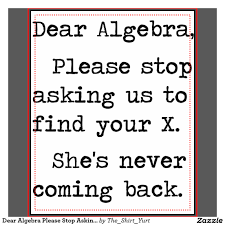
\includegraphics[width=0.23\textwidth]{algebrajoke.png}
  \end{center}
\end{wrapfigure}

Вы, наверняка знаете, что такое вектор --- объект в некотором пространстве. Можно мыслить о векторах как о ``стрелочках'', если мы говорим о пространстве положений. Этот вектор можно разложить по базису. Обычно мы работаем в нашем родном трёхмерном пространстве, где базис --- это единичные вектора осей $\mathbf{e}_x$, $\mathbf{e}_y$, $\mathbf{e}_z$. Над векторами можно делать преобразования, которые задаются матрицами преобразований. Давайте перенесёмся на плоскость и рассмотрим некоторые примеры.

\begin{center}
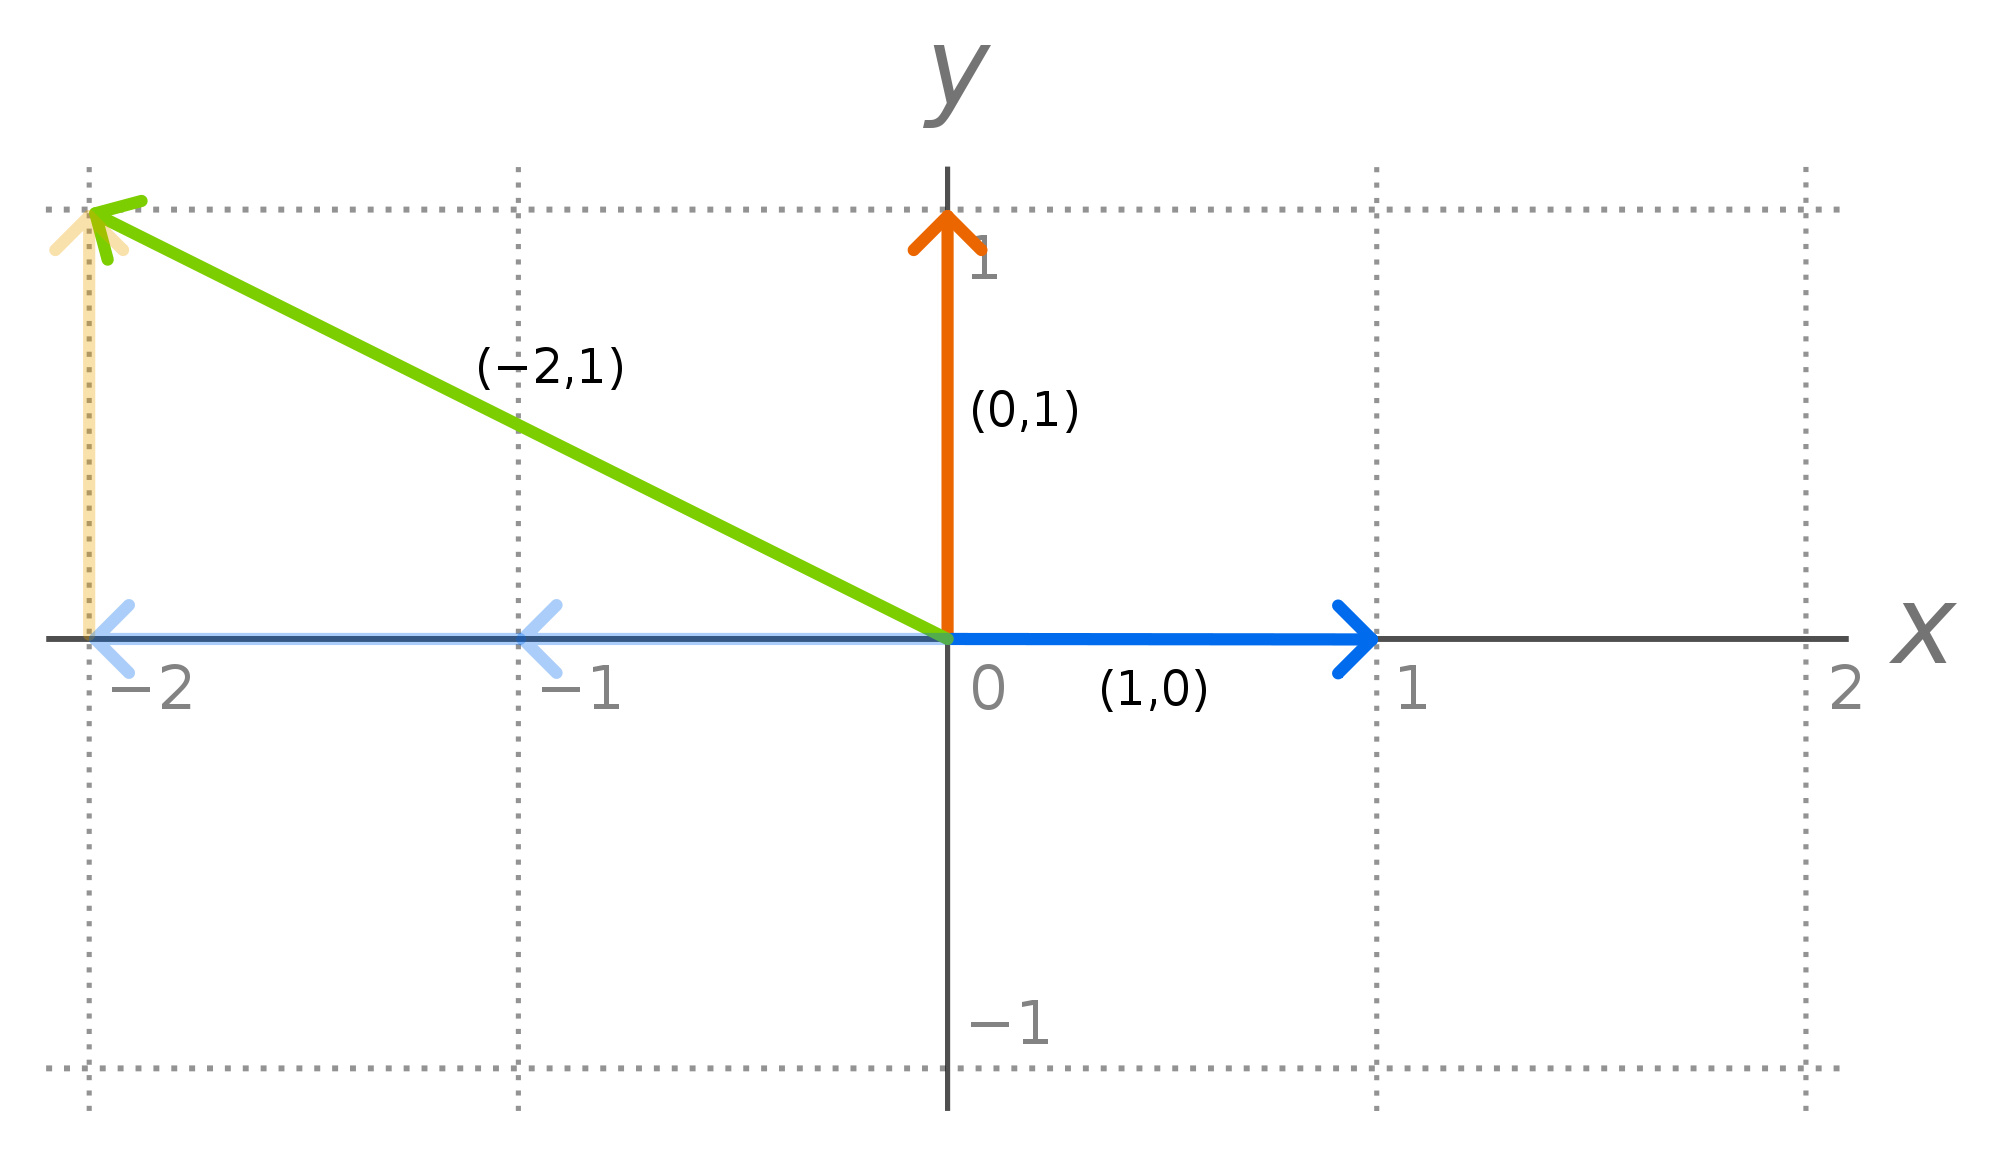
\includegraphics[scale=0.15]{basis.png}
\end{center}

Вектор на плоскости задаётся двумя числами, которые отражают его разложение по базисным векторам. Далее мы будем рассматривать только ортонормированные базисы: то есть за основу взяты два вектора с единичной длиной и перпендикулярные друг другу. На рисунке изображены несколько векторов и записано их разложение по базисным векторам.

На векторах определены простые операции. Пусть имеются векторы $\mathbf{u} = (u_x, u_y)$ и $\mathbf{v} = (v_x, v_y)$. Векторы можно складывать и вычитать $(u_x \pm v_x, u_y \pm v_y)$, умножать на число: $\lambda \mathbf{u} = (\lambda u_x, \lambda u_y)$.

Введём важное понятие {\bf скалярного произведения}. Если есть два вектора $\mathbf{u} = (u_x, u_y)$ и $\mathbf{v} = (v_x, v_y)$, то их скалярное произведение обозначается $(\mathbf{u}, \mathbf{v}) = u_x v_x + u_y v_y$. В двумерном и трёхмерном пространстве скалярное произведение имеет очень простой и понятный смысл. который следует из формулы $(\mathbf{u}, \mathbf{v}) = |\mathbf{u}| |\mathbf{v}| \cos \theta$, где $\theta$ --- угол между векторами. Получается, что скалярное произведение равно произведению длин векторов на косинус угла между ними.

{\bf Задача}: чему равны скалярные произведения $(\mathbf{e}_x, \mathbf{e}_y)$, $(\mathbf{e}_x, \mathbf{e}_x)$, $(\mathbf{e}_y, \mathbf{e}_y)$?

{\bf Задача}: пусть задан вектор $\mathbf{v} = (v_x, v_y)$. Чему равны произведения $(\mathbf{v}, \mathbf{e}_x)$, $(\mathbf{v}, \mathbf{e}_y)$? Каков их смысл?

{\bf Задача}: опишите семейство векторов, ортогональных (перпендикулярных) вектору $(-1, 1)$? 

{\bf Задача}: докажите, что $(\mathbf{v}, \mathbf{v}) = |\mathbf{v}|^2$.

{\bf Задача}: что происходит со скалярным прозведением при домножении одного из векторов на $-1$? Как это согласуется со свойствами косинуса? Сделайте рисунок, чтобы понять.

Важное замачание: любой вектор на плоскости выражается в виде {\bf линейной комбинации} векторов $\mathbf{e}_x$, $\mathbf{e}_y$: $\mathbf{v} = v_x \mathbf{e}_x + v_y \mathbf{e}_y.$ Линейная комбинация потому так называется, что вектор --- сумма базисных с коэффициентами.

{\bf Задача}: используя определение нормы векора через скалярное произведение, опишите множество коэффициентов $v_x$ и $v_y$ таких, что для вектора $\mathbf{v} = v_x \mathbf{e}_x + v_y \mathbf{e}_y$, $|v| = 1$. Тривиальный ответ, не правда ли?

\begin{wrapfigure}{r}{0.5\textwidth}
  \begin{center}
    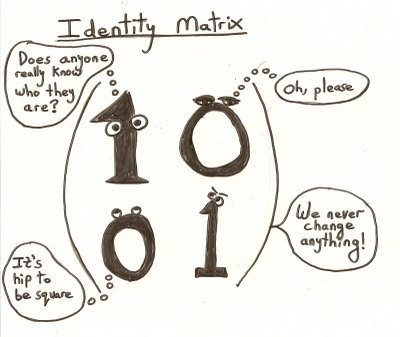
\includegraphics[width=0.40\textwidth]{algebrajoke2.jpg}
  \end{center}
\end{wrapfigure}

Теперь поговорим о таком объекте как {\bf матрица}. Для начала, на матрицу можно смотреть просто как на таблицу чисел размера $n \times m$. Матрицы окружают нас везде в жизни: изображение на компьютере --- это матрица (три матрицы для интенсивностей каждого из цветов RGB), карта дорог между городами --- это матрица (для каждой пары городов элемент матрицы говорит, сколько времени требется для проезда между городами). Здесь мы будем говорить про матрицы $2 \times 2$. Итак, вот она, матрица! $$M = \begin{pmatrix} M_11 & M_22 \\ M_21 & M_22\end{pmatrix}.$$
Это самый общий вид матрицы, $M_11$ и так далее --- это её элементы. Главный прикол матрицы в том, что её можно умножать на вектор...

Теперь мы готовы приступить к следующему очень важному объекту: {\bf операторам}. Не вдаваясь в глубокие математические тонкости, можно сказать, что оператор $\hat{A}$, если базис фиксирован, задаётся некоторой матрицей $A$. Если оператор $\hat{A}$ действует на двумерном пространстве, то его матрица $A$ размера $2 \times 2$. Операторы действуют на вектор, в результате получается какой-то другой вектор. Как именно оператор действует на вектор? Вектор умножается на матрицу оператора. Как происходит умножение матрицы на вектор?

\begin{gather*}
\hat{A} \mathbf{v} = A \mathbf{v} = \begin{pmatrix}A_xx & A_xy \\ A_yx & A_yy \end{pmatrix} \begin{pmatrix} v_x \\ v_y\end{pmatrix} = \begin{pmatrix} A_xx v_x + A_xy v_y \\ A_yx v_x + A_yy v_y\end{pmatrix} = \begin{pmatrix} v_x' \\ v_y'\end{pmatrix} 
\end{gather*}

По-простому формулу запоминают так: берём $i$-тую строчку матрицы, умножаем её почленно на столбик вектора и пишем это в $i$-тый элемент результата.

Есть и более глубинное понимание этой формулы, которое крайне важно. Элемент матрицы $A_xx$ --- это то, какой вклад даст $v_x$ в $v_x'$, $A_xy$ --- какой вклад даёт $v_x$ в $v_y'$, и так далее. То есть, оно говорит, {\bf в какой степени} те или иные координаты предыдущего вектора влияют на координаты следующего.

{\bf Задание}: что такой за оператор с матрицей $$\begin{pmatrix} 1 & 0 \\ 0 & 1 \end{pmatrix}?$$

{\bf Задание}: что за оператор такой с матрицей $$\begin{pmatrix} 1 & 0 \\ 0 & -1 \end{pmatrix}?$$

{\bf Задание}: что это за оператор такой с матрицей $$\begin{pmatrix} \cos \varphi & \sin \varphi \\ -\sin\varphi & \cos \varphi \end{pmatrix}?$$

Операторы можно перемножать между собой. Геометрически это обозначает последовательное действие на пространство. Например, пусть есть прямая $y = x$. Как написать оператор отражения относительно этой прямой? Утверждается, что $$A_{\mbox{отражение относительно} y = x} = A_{\pi / 4} A_{\mbox{отражение относительно} x = 0} A_{-\pi/4},$$ где $A_{\pm \pi / 4}$ --- операторы поворотов против и по часовой стрелки(е).

{\bf Задание}: покажите это!

Теперь вопрос: как записать это в виде одной матрицы, а не в виде трёх? Вначале у нас было что-то вроде $$\begin{pmatrix} \sqrt{2} / 2 & \sqrt{2} / 2 \\ - \sqrt{2} / 2 & \sqrt{2} / 2\end{pmatrix} \begin{pmatrix} -1 & 0 \\ 0 & 1 \end{pmatrix} \begin{pmatrix} \sqrt{2} / 2 & -\sqrt{2} / 2 \\  \sqrt{2} / 2 & \sqrt{2} / 2\end{pmatrix} = \mbox{отражение относительно}\;y = x.$$

{\bf Задание}: считая, что $AB v = Cv$, где $v$ --- некоторый произвольный вектор, запишите, как производится вычисление $C = AB$.

{\bf Задание}: используя это знание, отыщите матрицу инверсии относительно оси $y = x$.

Наконец, нам важно понятие {\bf собственного значения} оператора. Что это такое? Пусть существуют векторы, для которых $\hat{A} \mathbf{v} = \lambda \mathbf{v}$. То есть оператор на некоторый вектор действует всего лишь растяжением. Тогда число $\lambda$ называется собственным значением оператора.

Как искать собственные значения операторов? Из уравнения $\hat{A} \mathbf{v} = \lambda \mathbf{v}$ следует $(\hat{A} - \lambda) \mathbf{v} = 0$. Очевидно, что если какой-то $v$ решает это уравнение, то и любой $cv$ решает --- домножение на константу ничего не поменяет. Это значит, что два уравнения выше (одно векторное есть два скалярных) должны быть зависимы --- одно есть другое, умноженное на число. Это эквивалентно тому, что $\det (A - \lambda) = 0$, где $\lambda$ обозначает теперь единичную матрицу, умноженную на $\lambda$.

{\bf Задание}: получите формулу для определителя матрицы $B$ в двумерном случае, взяв за требование, что оба уравнения $B \mathbf{v} = 0$ (два скалярных) зависимы тогда и только тогда, когда $\det B = 0$.

{\bf Задание}: найдите определители всех матриц, которые упоминались в этом занятии.

Ещё одно важное определение, которое нужно сказать, это унитарный оператор. Унитарный оператор --- это такой, у которого модуль всех корней равен единице. Поворот, отражение, тождественное преобразование --- всё это унитарные операторы.

Раньше мы рассматривали векторы, компонентами которых являются вещественные числа. Для наших нужд придётся сказать, что компоненты векторов, а также элементы матриц операторов --- комплексные числа. По сути, всё, что мы определили раньше работает, но пару определений нужно уточнить. 

Во-первых, меняется определение скалярного произведения (проекции). Пусть снова мы работаем в ортонормированном базисе, т.е. $(\mathbf{e}_1, \mathbf{e}_1) = (\mathbf{e}_2, \mathbf{e}_2) = 0$, $\mathbf{e}_1, \mathbf{e}_2 = 1$. Если есть векторы $\mathbf{u} = u_1 \mathbf{e}_1 + u_2 \mathbf{e}_2$, $\mathbf{v} = v_1 \mathbf{e}_1 + v_2 \mathbf{e}_2$, то скалярное произведение равняется $(u, v) = u^* v = u_1^* v_1 + u_2^* v_2$. То есть компоненты левого вектора перед взятием скалярного произведения нужно сопрячь. Скалярное произведение уже более не имеет такого простого геометрического смысла, но если оно равно нолю, то по определению мы говорим, что векторы ортогональны.

{\bf Задание}: после расширения поля до комплексых чисел, поворот имеет собственные векторы. Найдите их.

{\bf Задание}: вычислите скалярное произведение векторов $\mathbf{v} = (1 + i, 3 - 2 i)$ и $\mathbf{u} = (4, -i)$.

{\bf Задание***}: докажите, что для унитарного оператора $(Au, v) = (u, Av)$ (это можно брать за определение).
\section*{Тема 7: пара слов о квантовой механике}
\begin{wrapfigure}{r}{0.5\textwidth}
  \begin{center}
    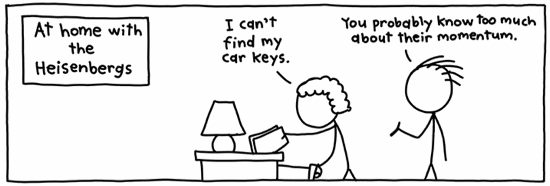
\includegraphics[width=0.40\textwidth]{quantumjoke1.png}
  \end{center}
\end{wrapfigure}
Сразу хочу предупредить: всё, что будет далее написано, не претендует на полноту изложения квантовой механики. Здесь будет рассказан лишь самый минимум, который нам нужен для понимания работы квантового компьютера (в общих чертах) и алгоритма Шора.

Теперь, когда мы что-то узнали о линейной алгебре пора поговорить о квантовой системе. Возможно, что-то будет звучать слишком абстрактно, но я постараюсь привести примеры.

\subsection*{Об измерениях}
Итак, в предыдущей теме мы говорили про базисные вектора и говорили не зря. Рассмотрим {\bf квантовую систему}, которая имеет два состояния, по традиции обозначающиеся $\Ket{0}$ и $\Ket{1}$. Состоянием может быть, например, энергетический уровень электрона в атоме (заставьте меня рассказать про атом Водорода) или спин свободного электрона (и рассказать про спин). Фишка квантовой механики в том, что система может находиться как в этих состояниях, так и в их некоторой смеси, которую называют {\bf суперпозицией}.

Общий вид состояния системы записывается как $\psi = \alpha \Ket{0} + \beta \Ket{1}$, где $\alpha$ и $\beta$ --- комплексные числа. Накладывается дополнительное условие $|\alpha|^2 + |\beta|^2 = 1$, смысл которого станет ясен чуть позже. Числа $\alpha$ и $\beta$ называются амплитудами состояний. Важно понять, что $\Ket{0}$ и $\Ket{1}$ --- это просто полные аналоги базисных векторов $\mathbf{e}_x$ и $\mathbf{e}_y$. Эти состояния задают базис в двумерном пространстве состояний системы так же, как и $\mathbf{e}_x$ и $\mathbf{e}_y$ задавали базис в двумерном пространстве положений. Получается, что амплитуды --- это аналоги $v_x$ и $v_y$ --- это {\bf проекции} состояния $\psi$ на базисные векторы $\Ket{0}$ и $\Ket{1}$.

Важный вопрос квантовой механики --- это процесс измерения. Пусть состояния $\Ket{0}$ (вниз) и $\Ket{1}$ (вверх) --- состояния электрона с определённым спином, вверх и вниз. Согласно Копенгагенской интерпретации, происходит следующее: когда квантовая система взаимодействует с внешним классичесим измерительным прибором (который каким-то образом измеряет спин), прибор всегда получит {\bf только} вверх или вниз (и никогда не что-то посередине). То есть, несмотря на то, что система находится в смеси состояний со спином $\pm 1$, измерение даёт определённый результат. При чём же здесь амплитуды $\alpha$ и $\beta$?

Оказывается, что прибор измерит спин ``вниз'' с вероятностью $|\alpha|^2$ и спин ``вверх'' с вероятостью $|\beta|^2$ (ясно, почему сумма должна быть равной 1?).

Важно: прибор {\bf испортит} нашу систему. После того, как произолшо измерение, состояние коллапсирует. Это означает, что если прибор намерил спин ``вниз'', то сразу после измерения система окажется в состоянии $\Ket{0}$ и дальше будет медленно эволюционировать их него. То есть, система коллапсирует в то состояние, которое было обнаружено классическим прибором.

\subsection*{Об эволюции}
\begin{wrapfigure}{r}{0.5\textwidth}
  \begin{center}
    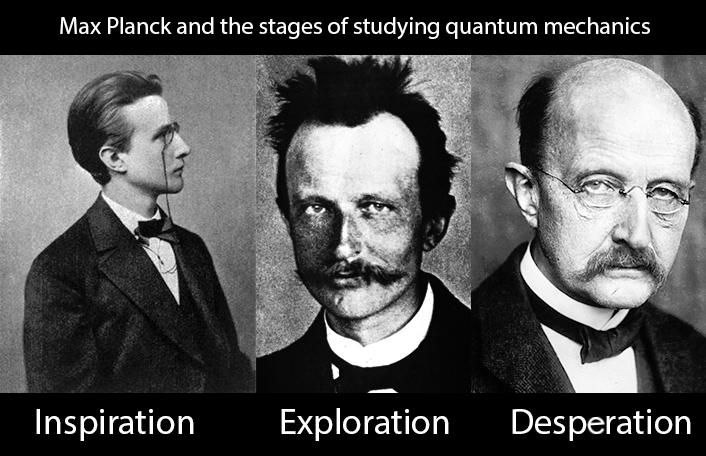
\includegraphics[width=0.40\textwidth]{quantumjoke2.png}
  \end{center}
\end{wrapfigure}
Квантовая механика, как и обычная механика, описывает эволюцию системы. В данном случае эволюционируют амплитуды (а вместе с ними вероятности) тех или иных состояний. В каждый конкретный момент времени система описывается значениями амплитуд $\alpha(t)$ и $\beta(t)$. Так как эти амплитуды --- это коэффициенты в разложении по базисным состояниям, то эволюционируют именно они. Пусть в начальный момент система находилась в состоянии $\alpha(0)$, $\beta(0)$. Какова связь между старыми и новыми коэффициентами? Вы уже догадались, нужно домножить на матрицу! $$\Ket{\psi(t)} = \hat{U}(t) \Ket{\psi(0)}.$$ Оператор $\hat{U}$ называется {\bf оператором эволюции}, а матрица $U$ --- матрица эволюции, которая связывает коэффициенты разложения старые и новые. Конкретный вид оператора эволюции зависит от системы и базиса состояний.

\begin{wrapfigure}{r}{0.5\textwidth}
  \begin{center}
    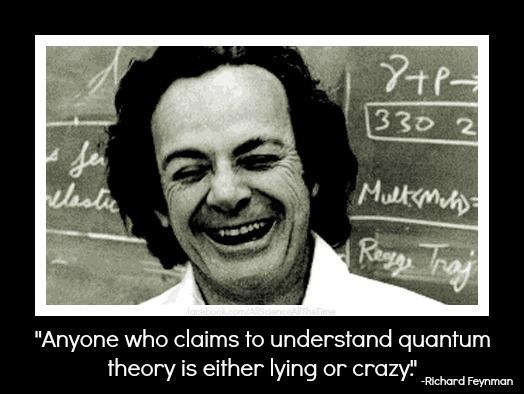
\includegraphics[width=0.40\textwidth]{quantumjoke3.jpg}
  \end{center}
\end{wrapfigure}
Здесь было сделано очень важное утверждение! Эволюция квантовой системы {\bf линейна}! То есть, новые коэффициенты всегда выражаются через старые линейно, то есть они стоят там всегда в первой степени, и вся эволюция выражается просто умножением на матрицу. Отсюда следует, что оператор $\hat{U}$ --- унитарный (почему?). Правильно, иначе бы он растягивал вектора, нарушая свойство $|\alpha|^2 + |\beta|^2 = 1$.

Квантовая механика работает таким образом: сначала можно подготовить систему в состоянии с определённым спином, например, вниз: $\Ket{0}$. Потом, зная параметры системы и время эволюции $t$, можно в принципе вычислить оператор эволюции $\hat{U}$ и найти, в каком состоянии (с камими амплитудами) будет система через время $t$. А амплитуды эти проявляют себя как вероятности получения того или иного значения спина при измерении.
{\bf Задача}: для матриц $\sigma_x = \begin{pmatrix} 0 & 1 \\ 1 & 0\end{pmatrix}$, $\sigma_y = \begin{pmatrix} 0 & -i \\ i & 0\end{pmatrix}$, $\sigma_z = \begin{pmatrix} 1 & 0 \\ 0 & -1\end{pmatrix}$ найдите собственные векторы и соответствующие им собственные значения.

Матрицы наверху называются матрицами Паули --- матрицы спина (внутреннего магнитного момента). Вектор, который является собственным, например, для $\sigma_x$, при измерении спина вдоль оси $x$ будет всегда давать одно значение.

\subsection*{О кубитах}
\begin{wrapfigure}{r}{0.5\textwidth}
  \begin{center}
    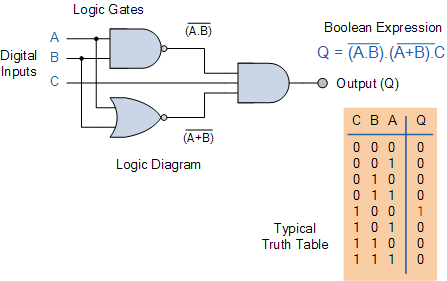
\includegraphics[width=0.40\textwidth]{logic.png}
  \end{center}
\end{wrapfigure}
До сих пор мы не касались темы самого, собственно, квантового компьютера. Основным элементом классического компьютера являются регистры, которые в себе содержат какое-то число. Для простоты будем считать, что регистр хранит в себе $0$ или $1$ и называется битом. Квантовым аналогом бита является кубит --- когда обычный бит может находиться {\bf только} в состояниях $\Ket{0}$ и $\Ket{1}$, квантовый же бит (кубит) может находиться в любой произвольной суперпозиции (описанной выше) и может эволюционировать со временем под действием унитарного оператора.

На классическом компьютере биты формируют различные арифметические схемы, которые состоят из базовых логических элементов AND, OR, NOT, XOR и так далее. Типичная такая схема изображена на рисунке выше.

Логические элементы преобразуют сигналы, приходящие им на вход, и на их основе формируют определённый выход. Для квантового компьютера существует нечто подобное. Квантовое состояние (или несколько состояний) подаются на вход квантового вентиля (quantum gate). Квантовый вентиль --- это некое унитарное преобразование, которое реализуется на практике множеством способов. Квантовый вентиль преобразует входные состояния определённым образом.

Рассмотрим основные виды квантовых вентилей, которые нам пригодятся для алгоритма Шора.

\subsubsection*{Вентиль Адамара}
Принимая на вход один кубит, он действует на него унитарным оператором с матрицей $$\hat{H} = \frac{1}{\sqrt{2}} \begin{pmatrix}1 & 1 \\ 1 & -1 \end{pmatrix}.$$

{\bf Задание}: как вентиль Адамара действует на состояния $\Ket{0}$ и $\Ket{1}$?

{\bf Задание}: найдите собственные векторы и собственные значения вентиля Адамара. Правда, оператор унитарный?

\subsubsection*{Вентиль фазового сдвига}
Принимая на вход один кубит, он действует на него унитарным оператором с матрицей $$\hat{R}_{\varphi} = \begin{pmatrix}1 & 0 \\ 0 & e^{i \varphi}\end{pmatrix}.$$

{\bf Задание}: найдите действие вентиля фазового сдвига на состояния $\Ket{0}$ и $\Ket{1}$. Унитарный оператор?

{\bf Задание}: найдите собственные векторы и собственные значения вентиля.

\subsubsection*{Контролируемый вентиль}
Сначала поговорим про операторы, действующие на нескольких квантовых состояниях. Пусть у нас есть не 1, а $m$ состояний. Когда было одно состояние, мы говорили, куда оно переводит ноль и нуда оно переводит один. Поэтому была матрица $2 \times 2$. А теперь у нас $2^m$ комбинаций, которые могут переходить в другие $2^m$ комбинаций, и потому матрица будет размера $2^m \times 2^m$.

Этот вентиль, посмотрев на регистр (несколько квантовых состояний) что-то делает с одим состоянием на входе. Не очень явная формулировка. Нам нужен будет только такой контролируемый вентиль: пусть в контролирующем регистре есть $m$ квантовых состояний. Пусть есть оператор, действующий на $m$ состояниях. Пусть к тому же в этих регистрах записано не что-то там, а собственный вектор этого оператора (один из). Тогда этот оператор, увидев это собственное значение (так как оно по модулю $1$, то $\lambda = e^{i \varphi}$), действует на единственный контролируемый кубит ($m$ контролирующих и 1 контролируемый) как вентиль фазового поворота на угол $\varphi$. Также можно построить аналогичные операторы, которые будут поворачивать состояние на угол $2^n \varphi$ --- то есть на любую степень двойки.

\section*{Тема 8: наконец, о квантовой составляющей алгоритма Шора}
УРААААА!!!!111! Вот мы и дошли до алгоритма Шора. Честно говоря, я уже немного устал печатать :) Ладно, ближе к делу.

\subsection*{Квантовое преобразование Фурье}
Так, стоп, мы же говорили об алгоритме Шора. Ах, сначала нужно сделать кое-что важное, а именно разобраться с квантовым дискретным преобразованием Фурье. Мы будем обсуждать только медленный алгоритм.

Что делает квантовое преобразование Фурье? На вход ему подаётся набор из $n$ кубитов, которые находятся в некой суперпозиции возможных $2^n$ состояний (напишите их!) с коэффициентами $x_1$, $x_2$, $\ldots$, $x_n$. Алгоритм трансформуриует эту систему так, что при этих $2^n$ состояниях оказываются коэффициенты $y_i$, которые являются дискретным преобразованием Фурье коэффициентов $x_i$. Соль в том, что чтобы закодировать $N$ состояний, нам нужно лишь $\log_2 N$ кубитов и $\log_2^2 N$ квантовых ворот, то есть это преобразование делается практически мгновенно.

{\bf Задание}: докажите, что всё целиком преобразование Фурье унитарно (попробуйте найти его собственные числа).

Как мы будем делать его? Каждое из $2^n$ состояний из $n$ кубитов мы будем обозначать $\Ket{j_1 j_2 \ldots j_n}$, где $j_i = 0,\;1$. Ещё введём обозначение $0.j_l j_{l + 1} j_{l + 2}\ldots j_m = j_l / 2 + j_{l + 1} / 4 + \ldots + j_{m} / 2^{m - l + 1}.$ 

Тогда утверждается, что преобразование Фурье --- это перевод каждого из $2^n$ состояний в суперпозицию по правилу $$\Ket{j_1 j_2 \ldots j_n} \to \frac{1}{2^{n / 2}} \left(\Ket{0} + e^{2 \pi i 0.j_n} \Ket{1} \right) \left(\Ket{0} + e^{2 \pi i 0.j_{n - 1} j_n} \Ket{1}\right)\ldots\left(\Ket{0} + e^{2 \pi i 0.j_1 j_2\ldots j_n}\Ket{1}\right).$$

Почему это именно преобразование Фурье? 
\begin{gather*}
\Ket{j} \to \frac{1}{2^{n / 2}}\sum\limits_{k = 0}^{2^n - 1} e^{2 \pi i j k / 2^n}\Ket{k} = \frac{1}{2^{n / 2}}\sum\limits_{k_1 = 0}^1 \ldots \sum\limits_{k_n = 0}^1 e^{2 \pi i j \left(\sum\limits_{l = 1}^n k_l / 2^l \right)}\Ket{k_1 k_2\ldots k_n} = \frac{1}{2^{n / 2}}\sum\limits_{k_1 = 0}^1 \ldots \sum\limits_{k_n = 0}^1 \prod\limits_{l = 1}^n \left(e^{2 \pi i j k_l / 2^l} \Ket{k_l}\right) = \\ = \frac{1}{2^{n / 2}}\prod\limits_{l = 1}^n\left(\Ket{0} + e^{2 \pi i j / 2^l} \right) = \frac{1}{2^{n / 2}} \left(\Ket{0} + e^{2 \pi i 0.k_n} \Ket{1} \right) \left(\Ket{0} + e^{2 \pi i 0.k_{n - 1} k_n} \Ket{1}\right)\ldots\left(\Ket{0} + e^{2 \pi i 0.k_1 k_2\ldots k_n}\Ket{1}\right).
\end{gather*} 

В последнем преобразовании мы использовали периодичность экспонент.

Схема преобразования приведена на рисунке (справа опущены корни из двух):
\begin{center}
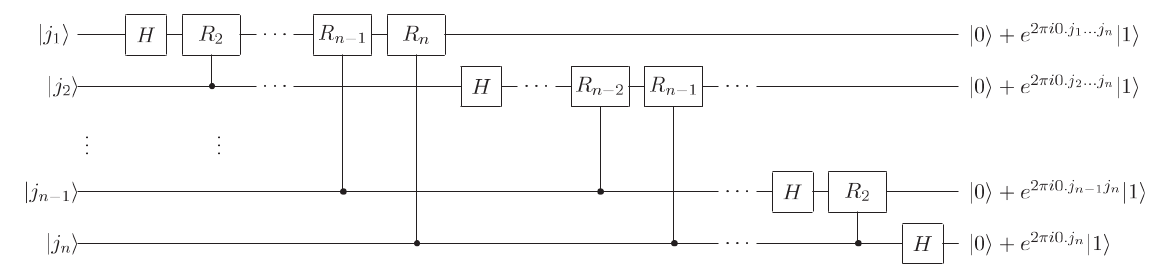
\includegraphics[scale=0.45]{qfft.png}
\end{center}

Вентиль $R_k$ на рисунке поворачивает $\Ket{1}$ на угол $2 \pi / 2^k$. Таким образом, после вентиля Адамара и $R_2$, получается состояние $\left(\Ket{0} + e^{2 \pi i 0.j_1}\Ket{1}\right)\Ket{j_2 j_3 \ldots j_n}$ (потому, что $e^{2 \pi i j_1 / 2} = \pm 1$). Применение $R_2$ вентиля превращает скобку в $\Ket{0} + e^{2 \pi i 0.j_1 j_2} \Ket{1}$. Применение всей череды $R_k$ делает из первого кубита $\Ket{0} + e^{2 \pi i 0.j_1 j_2 \ldots j_n}\Ket{1}$. В конце концов получаются скобки, которые нужны, но в перевёрнутом порядке. Унитарным образованием можно попереставлять пары кубитов и получить правильную последовательность скобок. Таким образом, теперь мы располагаем способом за $\mathcal{O}(n^2)$ вентилей делать преобразование Фурье вектора длины $2^n$.

\subsection*{Оценка фазы}
Следующая важная часть алгоритма Шора --- phase estimation. Поговорим о ней подробнее. Пусть имеется унитарный оператор $\hat{U}$ и собственный вектор $\Ket{u}$, собственное значение $e^{2 \pi i \varphi}$, фаза $\varphi$ нам неизвестна. Цель алгоритма --- определить фазу $\varphi$ с некоторой точностью, которая экспоненциально падает с числом задействованных в алгоритме кубитов. Для начала представим, что мы имеем оракула, который умеет подготавливать собственное состояние $\Ket{u}$ (регистр на множестве кубитов), а также умеет быстро действовать на это состояние оператором $\hat{U}^{2^j}$ для любого неотрицательного целого $j$ (то есть может быстро подействовать определёнными степенями оператора $\hat{U}$). Алгоритм оценки фазы нужен для многих квантовых алгоритмах, поэтому пока удобнее о нём думать без привязки к алгоритму Шора. В случае алгоритма Шора оракул превратится во что-то осязаемое.

Алгоритм использует два регистра. Первый регистр задаётся $t$ кубитами, которые все изачально находятся в состоянии $\Ket{0}$. Число $t$ опредетяет точность, с которой будет сделана оценка фазы $\varphi$. Второй регистр содержит столько кубитов, сколько нужно, чтобы задать состояние $\Ket{u}$.

Алгоритм состоит из двух частей. Первая часть выражена схемой, изображённой на рисунке.
\begin{center}
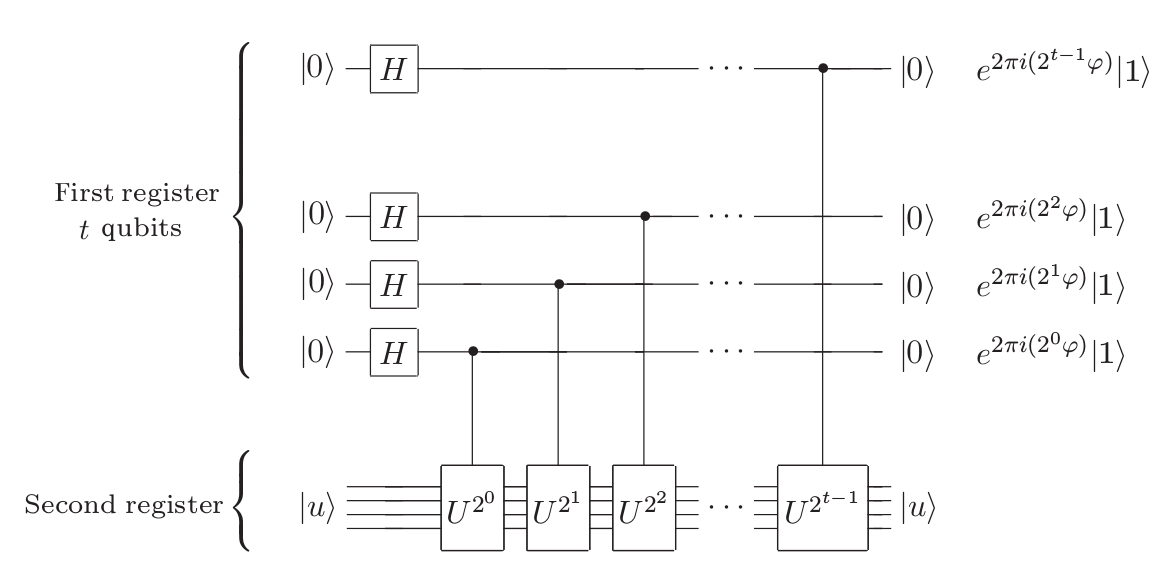
\includegraphics[scale=0.45]{schemephase.png}
\end{center}

Если учесть, что $\Ket{u}$ --- собственное состояние оператора $\hat{U}$ (а как действует степень оператора на собственный вектор?), то эта схема создаёт состояние $$\frac{1}{2^{t / 2}}\left(\Ket{0} + e^{2 \pi i 2^{t - 1}\varphi}\Ket{1}\right)\ldots\left(\Ket{0} + e^{2 \pi i 2^{0}\varphi}\Ket{1}\right) = \frac{1}{2^{t / 2}}\sum\limits_{k = 0}^{2^t - 1} e^{2 \pi i \varphi k}\Ket{k}.$$ Здесь под $\Ket{k}$ подразумевается определёное состояние $t$ кубитов (какое?). Затем нужно инвертировать кубиты, то есть поменять $1$ и $n$, $2$ и $n - 1$, и так далее.

{\bf Задание}: почему описанное выше преобразование унитарно? 

{\bf Задание}: как выглядит матрица преобразования Адамара одного кубита в виде оператора, действующего на систему из $n$ кубитов?

{\bf Задание}: запишите матрицу оператора инверсии $n$ кубитов.

Вторая стадия алгоритма --- применить обратное квантовое преобразование Фурье. По сути это прямое преобразование Фурье, но с вращениями на отрицательные фазы. Его мы уже умеем делать.

Чтобы наша интуиция работала выше, будем считать, что фаза $\varphi$ выражается в точности $t$ битами, $\varphi = 0.\varphi_1\ldots\varphi_t$ (почему так можно считать?). Тогда приведённая формула принимает вид (периодичность экспонент): 

$$\frac{1}{2^{t / 2}}\left(\Ket{0} + e^{2 \pi i 0.\varphi_{t}}\Ket{1}\right)\ldots\left(\Ket{0} + e^{2 \pi i 2^{0}0.\varphi_1\varphi_2\ldots\varphi_t}\Ket{1}\right).$$

Теперь настало время делать обратное преобразование Фурье. Но ведь формула выше --- это результат прямого преобразования Фурье над вектором $\Ket{\varphi} = \Ket{\varphi_1\varphi_2\ldots\varphi_t}$. Стало быть, обратное преобразование Фурье даст нам именно $\Ket{\varphi}$. Поэтому теперь мы можем изменять регистр $\Ket{t}$ и получать $\varphi$.

\subsection*{Собственно поиск порядка}
Научившись искать собственные значения унитарного оператора на квантовом компьютере, мы готовы к поиску порядка элемента, что является финальной точкой в алгоритме разложения числа $N$ на $p$ и $q$ (сам не верю, что я допечатал этот текст до этого места, а вы?). Итак, пусть мы хотим найти порядок элемента $x$ по модулю $N$, то есть наименьшее число $r$ такое, что $x^r = 1\;\mbox{mod}\;N$. Для этого мы будем применять алгоритм оценки фазы к оператору $\hat{U}\Ket{y} = \Ket{xy\;\mbox{mod}\;N}$. Имеется в виду, что если у нас есть $n$ кубитов, которые кодируют число $y$, то этот оператор переводит такое состояние в состояние, описывающее не число $y$, а число $xy\;\mbox{mod}\;N$.

{\bf Задание}: покажите, что состояния вида $\Ket{u_s} = \frac{1}{\sqrt{r}}\sum\limits_{k = 0}^{r - 1} e^{-2 \pi i s k / r}\Ket{x^k\;\mbox{mod}\;N}$ являются собственными для этого оператора с собственными значениями $\lambda_s = e^{2 \pi i s / r}$.

Супер! Получается, мы можем, используя алгоритм оценки фазы, измерять для любого $s$ отношение $s/r$, и таким образом находить $r$ --- порядок! Сколько нам потребовалось операций? Порядок группы $r$ не может быть больше $N$. Для хорошей оценки $r$ нам нужно брать порядка $\log_2 N$ регистров, и в итоге вся возня делается за $\log_2^3 N$ операций (давайте посчитаем?).

\subsection*{Ложка дёгтя}
Осталось сделать два важных замечания. Первое: как быстро искать большую степень оператора $\hat{U}$. На этот вопрос вы можете ответить сами --- это динамическое возведение в степень.

Кроме того, подготовить состояние $\Ket{u_s}$ невозможно! Его определение включает в себя неизвестный нам $r$. Как быть? 

{\bf Задание}: докажите, что $\frac{1}{\sqrt{r}}\sum\limits_{s = 0}^{r - 1}\Ket{u_s} = \Ket{1}$.

Таким образом, вместо $\Ket{u_s}$ мы будем скармливать в управляющий регистр просто состояние $\Ket{1}$ (как это в кубитах?). Это состояние --- это суперпозиция собственных состояний $\Ket{u_s}$. Сделав измерение один раз, мы найдём какое-то отношение $s / r$ для некоторого случайного $s$. Беда в том, что это отношение мы можем измерить лишь с некой точностью (у нас конечное число регистров). При этом мы знаем, что мы измеряем некую рациональную дробь! Поэтому (есть просто такая теорема), что при достаточном числе кубитов (хватит $\log_2^2 N$ мы сможем безошибочно определить, какая это именно дробь, и, соответственно, каков порядок $r$).
\end{document}